\documentclass[a4paper, 12pt]{article}

\usepackage{fontspec}
\usepackage{polyglossia}
\defaultfontfeatures{Ligatures=TeX}
\setdefaultlanguage{russian}
\setotherlanguage{english}
\setmainfont{Times New Roman}
\newfontfamily{\latinfont}{Times New Roman}
\newfontfamily{\cyrillicfont}{Times New Roman}
\newfontfamily{\cyrillicfonttt}{Courier New}

\usepackage{geometry}
\usepackage{amsmath}
\usepackage{amssymb}
\usepackage{amsfonts}
\usepackage{graphicx}
\usepackage{float}
\usepackage{wrapfig}
\usepackage{subcaption}
%\usepackage[caption=false]{subfig}
\geometry{right=20mm}
\geometry{left=20mm}
\geometry{top=20mm}
\geometry{bottom=20mm}

\usepackage{indentfirst}
\usepackage[outputdir=auxiliary]{minted}

\graphicspath{{../img/}}
\DeclareMathOperator{\R}{\mathbb{R}}
\DeclareMathOperator{\C}{\mathbb{C}}
\renewcommand{\Re}{\mathrm{Re}}
\renewcommand{\Im}{\mathrm{Im}}


\begin{document}
    \begin{titlepage}
    \begin{center}
        \textit{МИНИСТЕРСТВО ОБРАЗОВАНИЯ И НАУКИ\\
        РОССИЙСКОЙ ФЕДЕРАЦИИ}
        \vspace{1ex}

        федеральное государственное бюджетное образовательное учреждение\\
        высшего профессионального образования
        \vspace{1ex}

        \textbf{САНКТ-ПЕТЕРБУРГСКИЙ НАЦИОНАЛЬНЫЙ ИССЛЕДОВАТЕЛЬСКИЙ УНИВЕРСИТЕТ ИТМО}
        \vspace{13ex}

        Лабораторная работа №3\\
        <<Динамика нелинейных систем>>\\
        по дисциплине <<Моделирование технических систем>>\\
        \vspace{1em}
        Вариант 3\\
    \end{center}
    \vspace{14em}
    \begin{flushright}
        \noindent
        Выполнили:\\
        студенты гр. R4133c\\
        Борисов М. В.\\
        Симонов П.\\
        Мацуганов А. И.\\
        \vspace{1em}
        Преподаватель:\\
        Семенов Д. М.
    \end{flushright}
    \vfill
    \begin{center}
        \large{Санкт-Петербург}\\
        2021 г.\\
    \end{center}
\end{titlepage}

    \setcounter{page}{2}
    \setlength{\parindent}{0pt}

    \section*{Задание}
    Дана нелинейная система.
    \begin{equation*}
        \left\{
        \begin{aligned}
            \dot{x_1} &= -x_1\\
            \dot{x_2} &= rx_2 - x_2^3 + x_2^5
        \end{aligned}
        \right.
    \end{equation*}

    \begin{enumerate}
        \item Найти возможные бифуркации в системе
        \item Определить тип положений равновесия для всех значений бифуркационного параметра $r$
        \item Построить фазовые портреты линеаризованной и исходной линейной систем для каждого типа положения равновесия
    \end{enumerate}

    \section*{Решение}
    \begin{equation*}
        \left\{
        \begin{aligned}
            x_1 &= 0\\
            rx_2 - x_2^3 + x_2^5 &= 0
        \end{aligned}
        \right.
    \end{equation*}
    \begin{equation*}
        \left\{
        \begin{aligned}
            x_1 &= 0\\
            x_2\left( x_2^4 - x_2^2 + r \right) &= 0
        \end{aligned}
        \right.
    \end{equation*}
    \begin{equation*}
        \left\{
        \begin{aligned}
            x_1 &= 0\\
            x_2 &= 0;\, \pm \sqrt{\dfrac{1}{2}\left( 1 \pm \sqrt{1 - 4r} \right)}
        \end{aligned}
        \right.
    \end{equation*}

    Таким образом получаем следующие точки равновесия:\\\sloppy
    \begin{equation}
        (0, 0), \label{p1}
    \end{equation}
    \begin{equation}
        \left(0, \sqrt{\dfrac{1}{2}\left( 1 + \sqrt{1 - 4r} \right)}\right) \label{p2},\,\mbox{где } r \in \left[ -\infty, \dfrac{1}{4} \right]
    \end{equation}
    \begin{equation}
        \left(0, -\sqrt{\dfrac{1}{2}\left( 1 + \sqrt{1 - 4r} \right)} \right) \label{p3},\,\mbox{где } r \in \left[ -\infty, \dfrac{1}{4} \right]
    \end{equation}
    \begin{equation}
        \left(0, \sqrt{\dfrac{1}{2}\left( 1 - \sqrt{1 - 4r} \right)}\right) \label{p4},\,\mbox{где } r \in \left[ 0, \dfrac{1}{4} \right]
    \end{equation}
    \begin{equation}
        \left(0, -\sqrt{\dfrac{1}{2}\left( 1 - \sqrt{1 - 4r} \right)} \right)\label{p5},\,\mbox{где } r \in \left[ 0, \dfrac{1}{4} \right]
    \end{equation}

    При $r$ вне указанных диапазонов корни получаются комплексными.

    Якобиан:\\
    \begin{equation*}
        J=
        \begin{bmatrix}
            -1& 0\\
            0& 5x_2^4 - 3x_2^2 + r
        \end{bmatrix}
    \end{equation*}

    Собственные значения якобиана очевидны и лежат на диагонали.

    Для пар точек равновесия~(\ref{p2}),~(\ref{p3}) и~(\ref{p4}),~(\ref{p5}) якобиан будет одинаков в силу чётности степени $x_2$.

    Получаем три различных якобиана:
    \begin{equation}
        \label{J1}
        J_1=
        \begin{bmatrix}
            -1& 0\\
            0& r
        \end{bmatrix}
    \end{equation}
    \begin{equation}
        \label{J23}
        J_{2,3}=
        \begin{bmatrix}
            -1& 0\\
            0& \dfrac{5\left( \sqrt{1 - 4r} + 1 \right)}{4}^2 - \dfrac{3\sqrt{1 - 4r}}{2} + r - \dfrac{3}{2}
        \end{bmatrix}
    \end{equation}
    \begin{equation}
        \label{J45}
        J_{4,5}=
        \begin{bmatrix}
            -1& 0\\
            0& \dfrac{5\left( \sqrt{1 - 4r} - 1 \right)}{4}^2 + \dfrac{3\sqrt{1 - 4r}}{2} + r - \dfrac{3}{2}
        \end{bmatrix}
    \end{equation}
    Для~(\ref{J1}) положение равновесия имеет тип
    \paragraph*{Устойчивый узел} $r < 0 ,\,(\lambda_{1, 2} \in \R; \lambda_1\cdot\lambda_2 > 0))$\nopagebreak
    \begin{figure}[H]
        \begin{subfigure}{0.5\linewidth}
            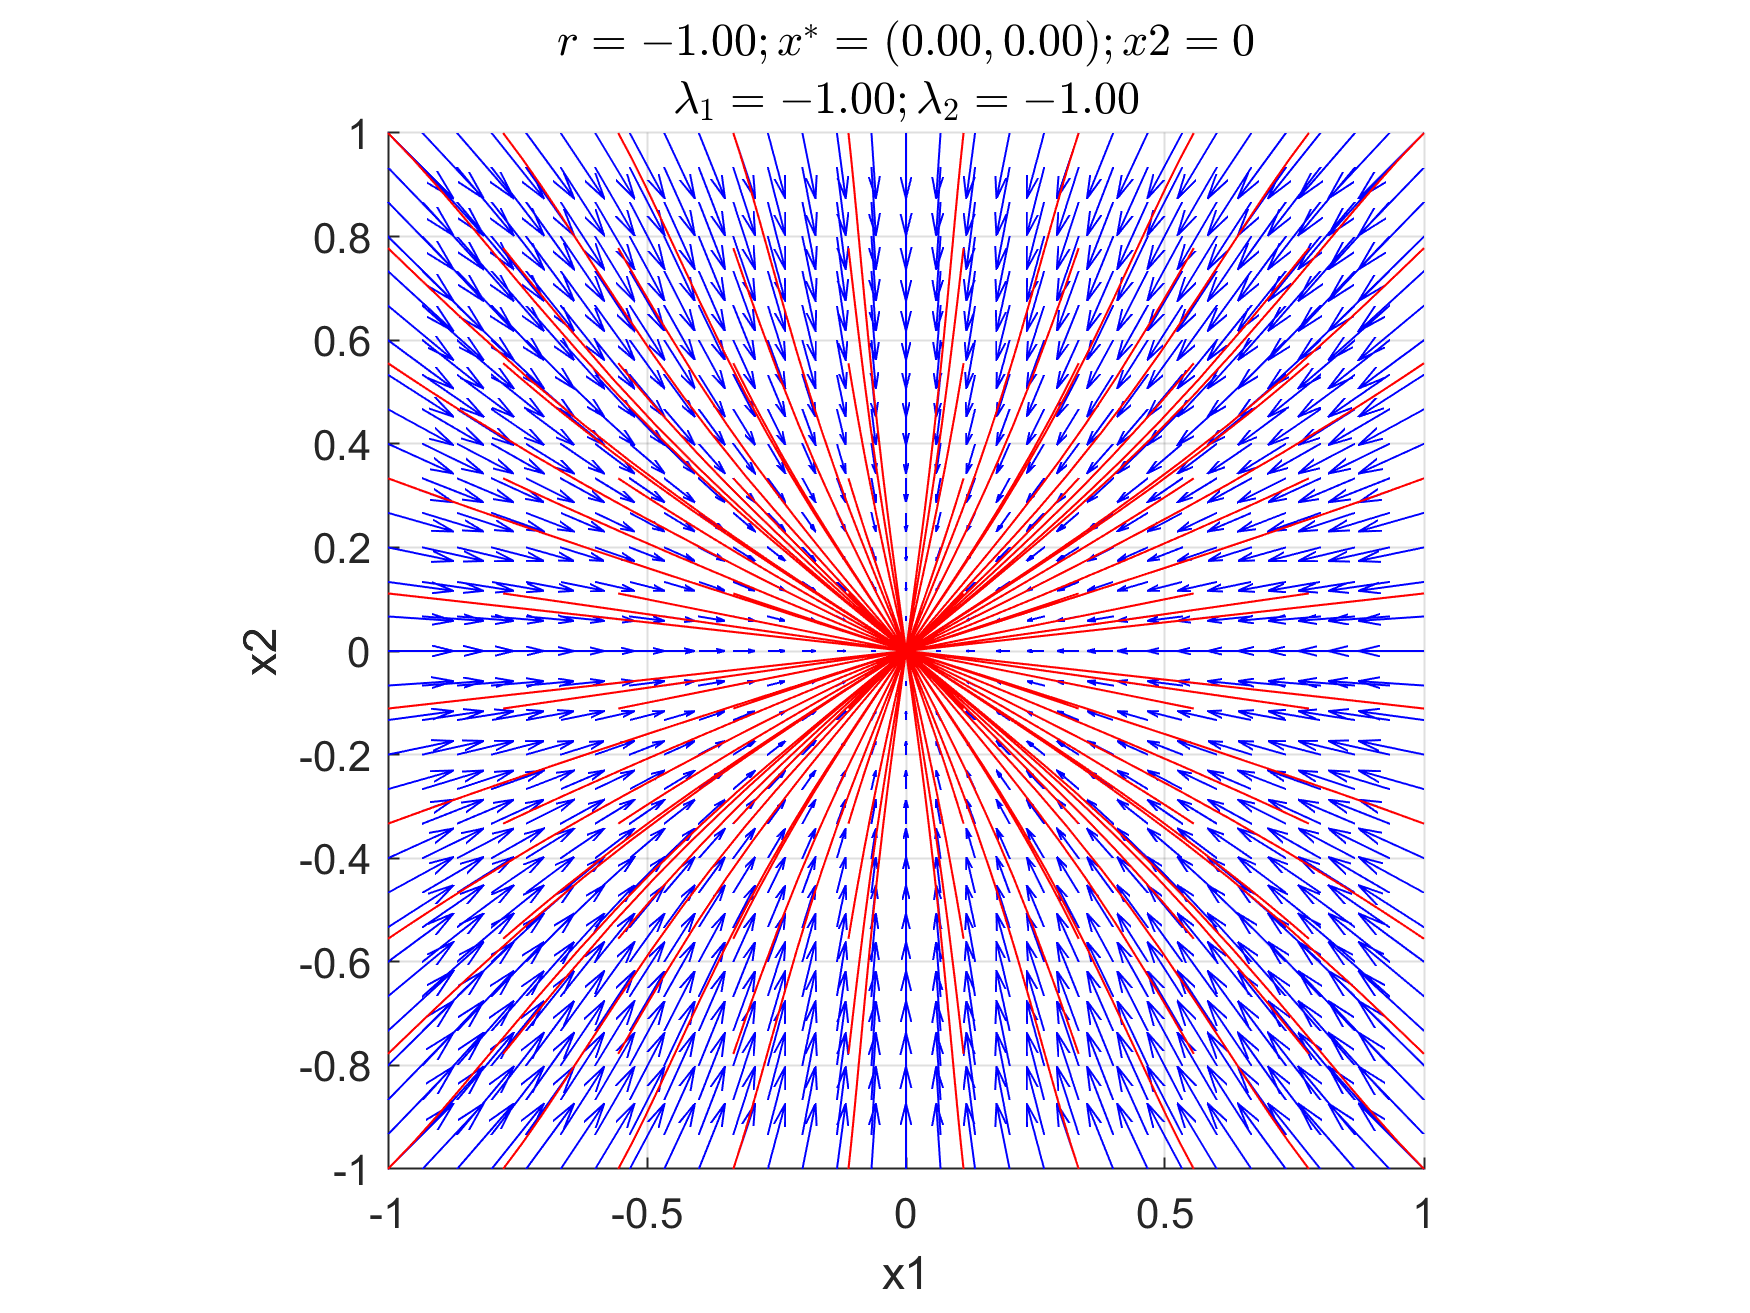
\includegraphics[width=\linewidth, trim={1cm, 0, 1cm, 0}, clip]{x1r-1.png}
            \caption{Исходная система}
        \end{subfigure}
        \begin{subfigure}{0.5\linewidth}
            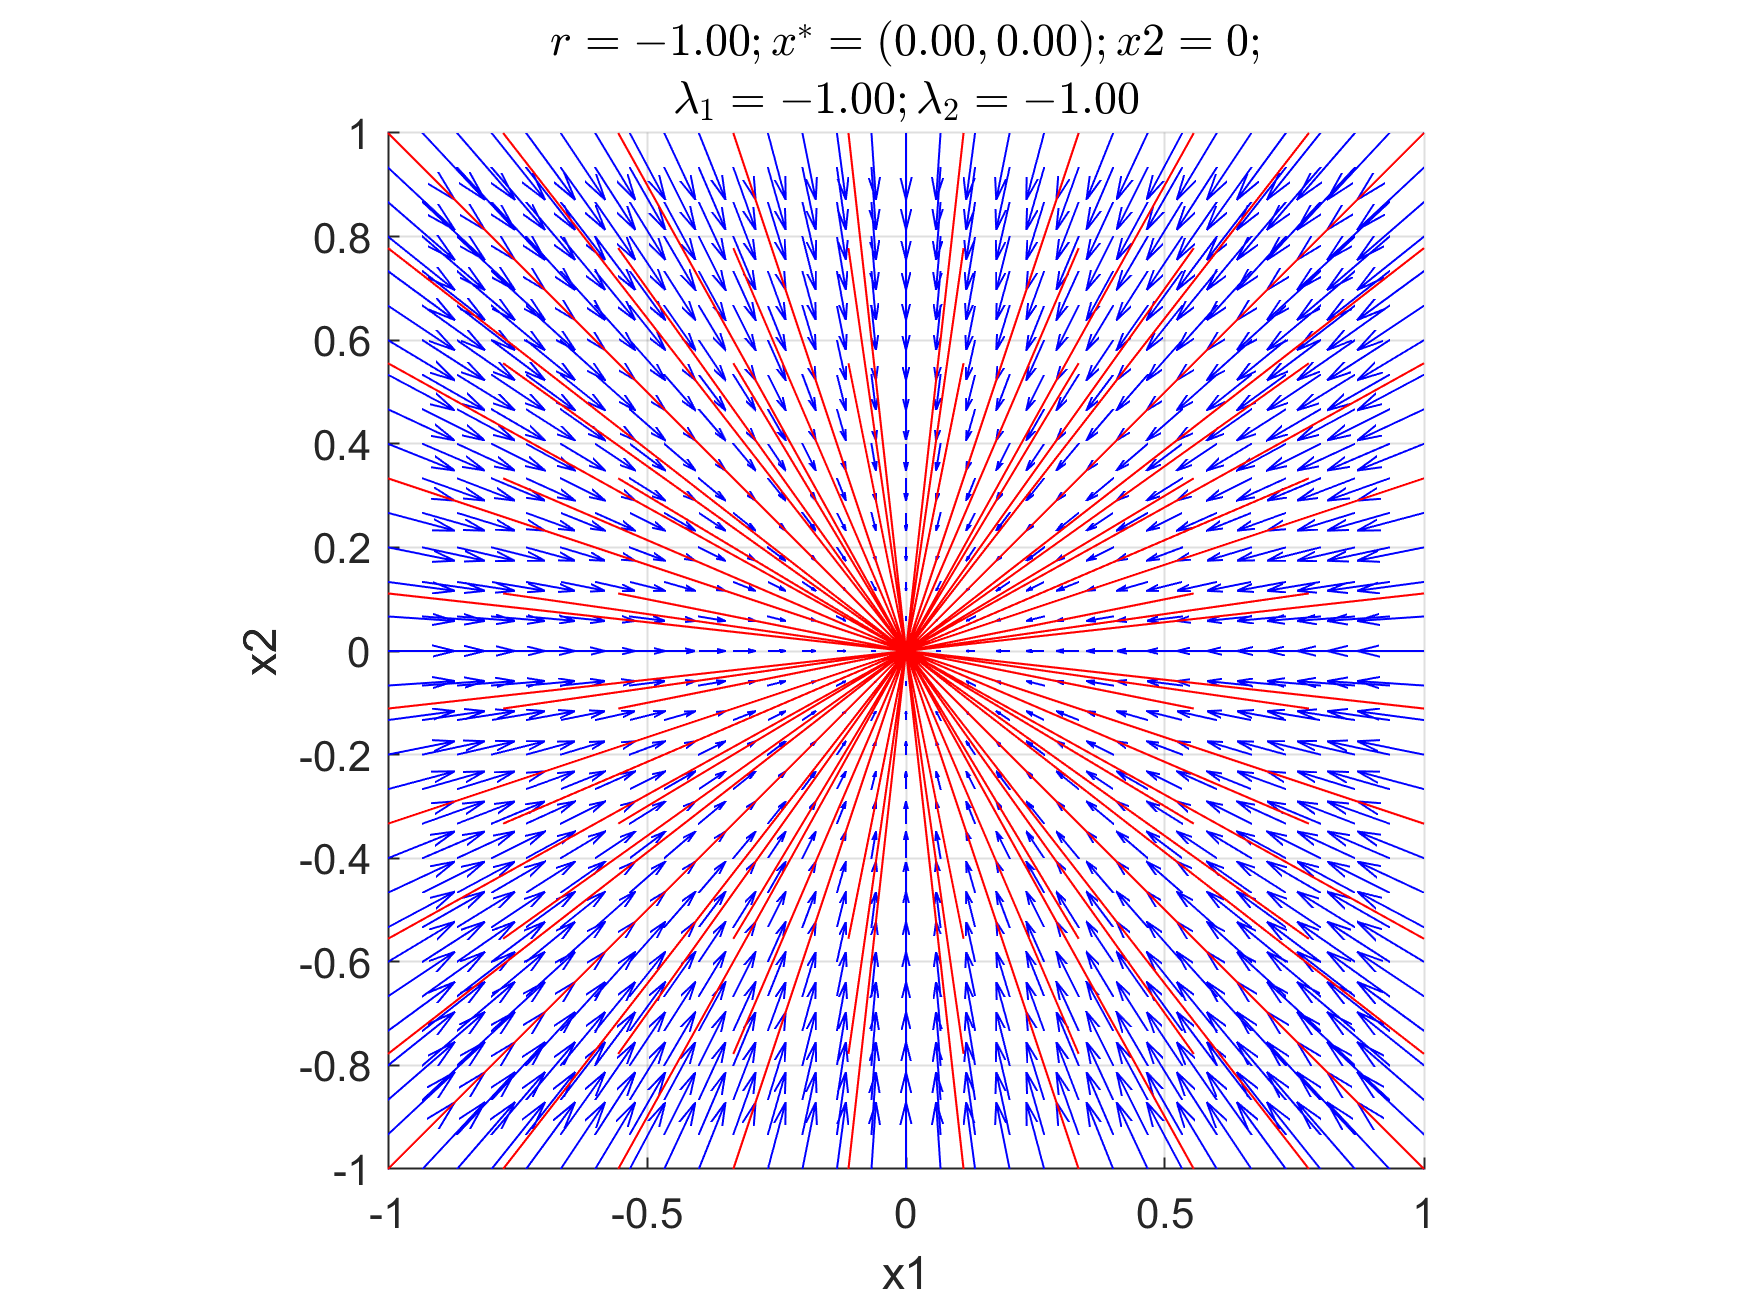
\includegraphics[width=\linewidth, trim={1cm, 0, 1cm, 0}, clip]{x1r-1-lin.png}
            \caption{Линеаризованная система}
        \end{subfigure}
        \caption{Фазовые диаграммы}
    \end{figure}

    \paragraph*{Седло} $r > 0 ,\,(\lambda_{1, 2} \in \R; \lambda_1\cdot\lambda_2 < 0))$\nopagebreak
    \begin{figure}[H]
        \begin{subfigure}{0.5\linewidth}
            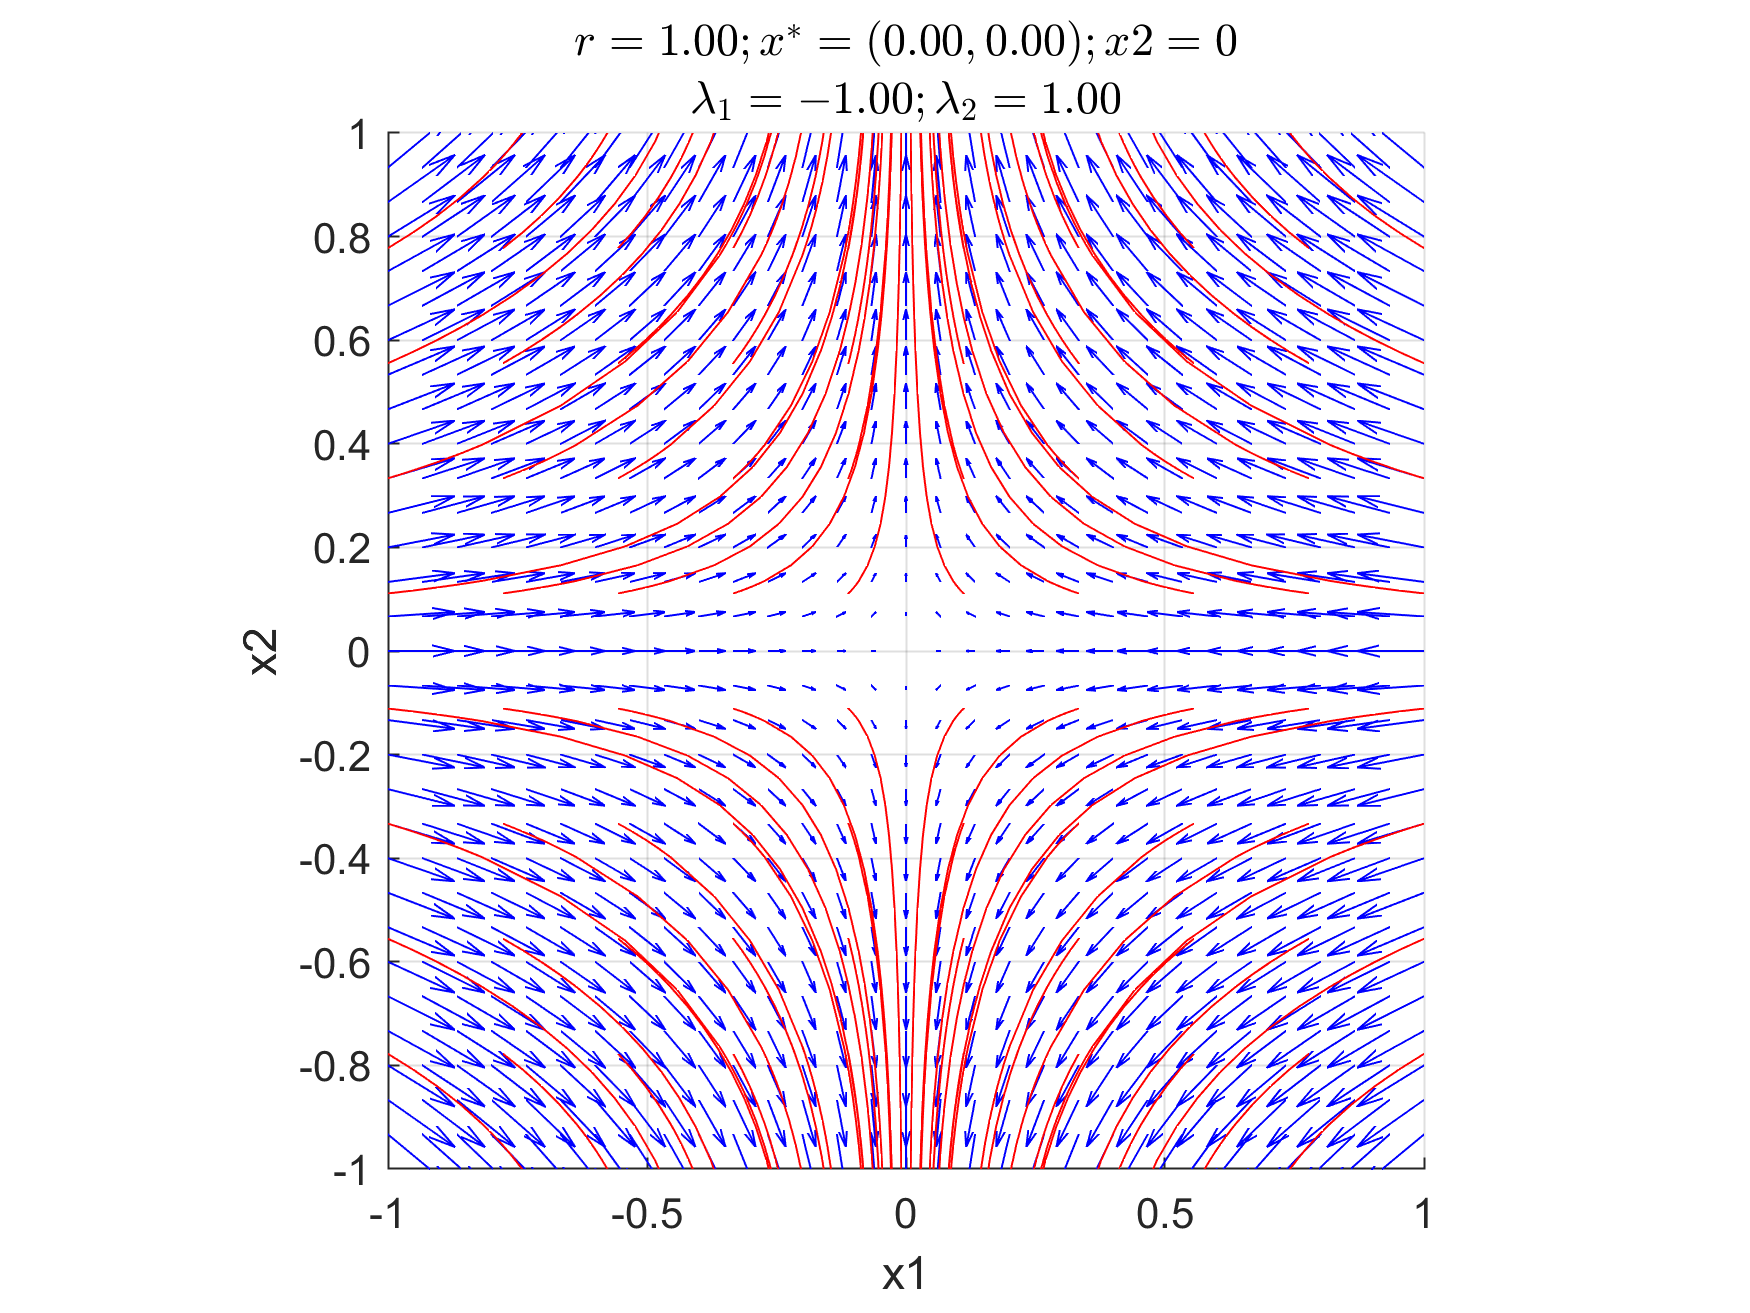
\includegraphics[width=\linewidth, trim={1cm, 0, 1cm, 0}, clip]{x1r1.png}
            \caption{Исходная система}
        \end{subfigure}
        \begin{subfigure}{0.5\linewidth}
            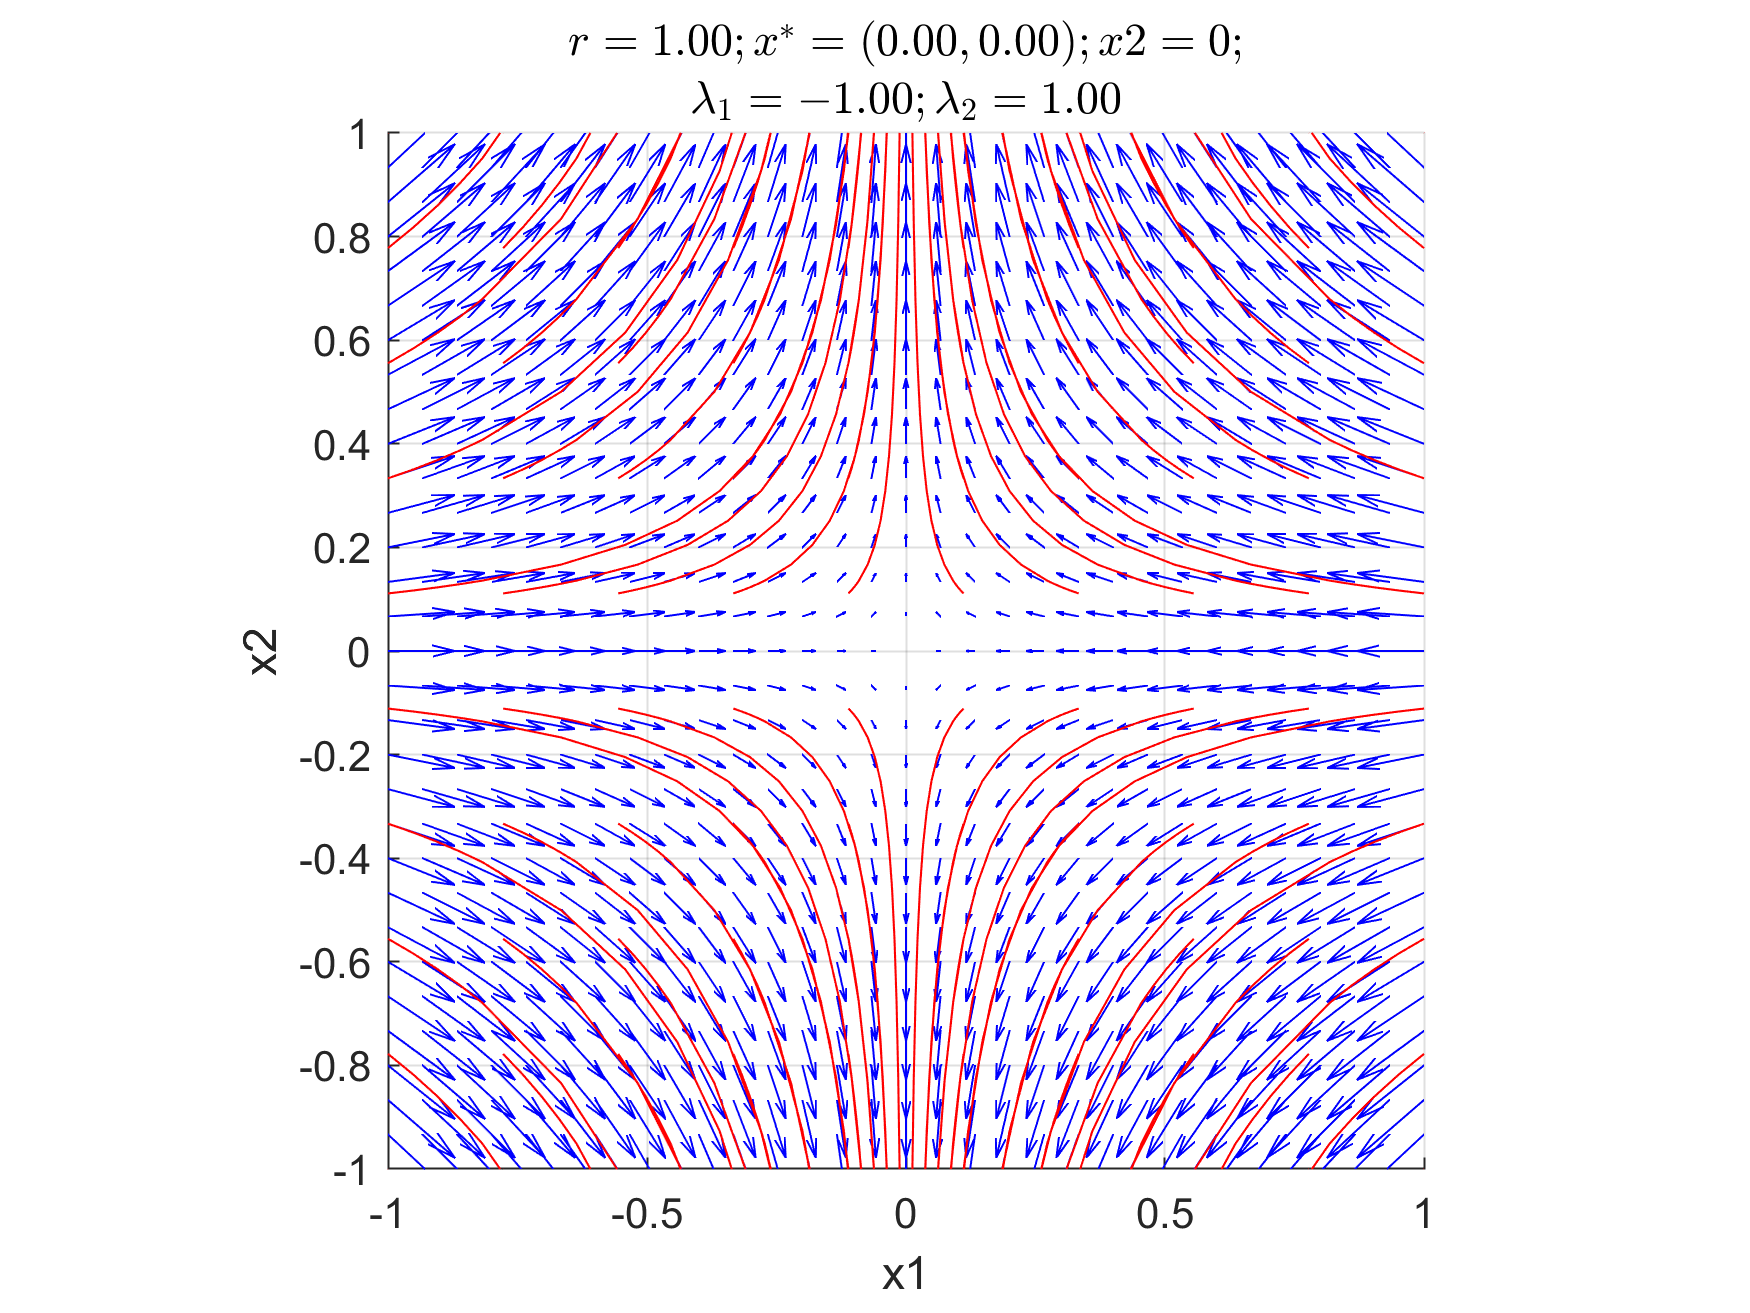
\includegraphics[width=\linewidth, trim={1cm, 0, 1cm, 0}, clip]{x1r1-lin.png}
            \caption{Линеаризованная система}
        \end{subfigure}
        \caption{Фазовые диаграммы}
    \end{figure}

    \paragraph*{Вырожденный случай} $r = 0 ,\,(\lambda_2 = 0 )$\nolinebreak
    \begin{figure}[H]
        \begin{subfigure}{0.5\linewidth}
            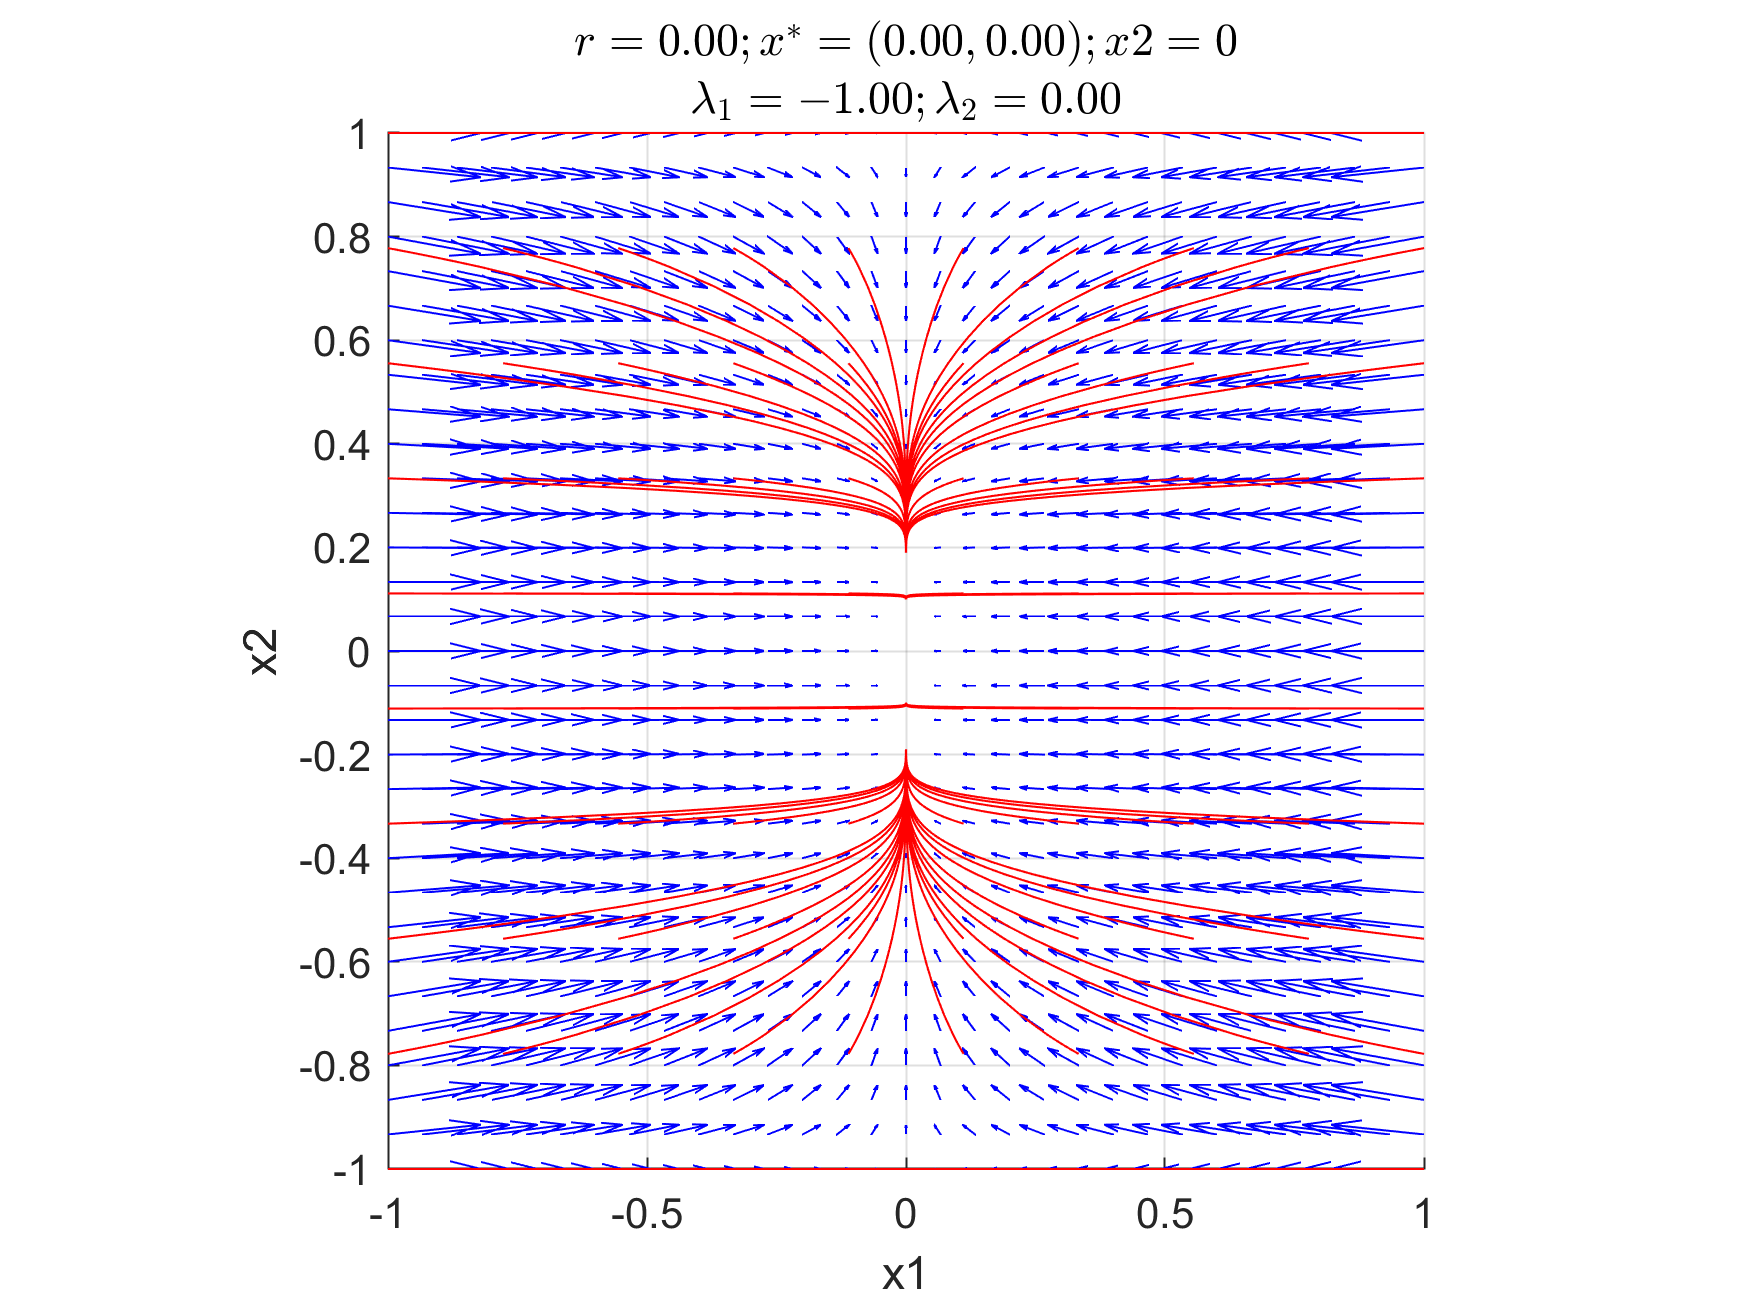
\includegraphics[width=\linewidth, trim={1cm, 0, 1cm, 0}, clip]{x1r0.png}
            \caption{Исходная система}
        \end{subfigure}
        \begin{subfigure}{0.5\linewidth}
            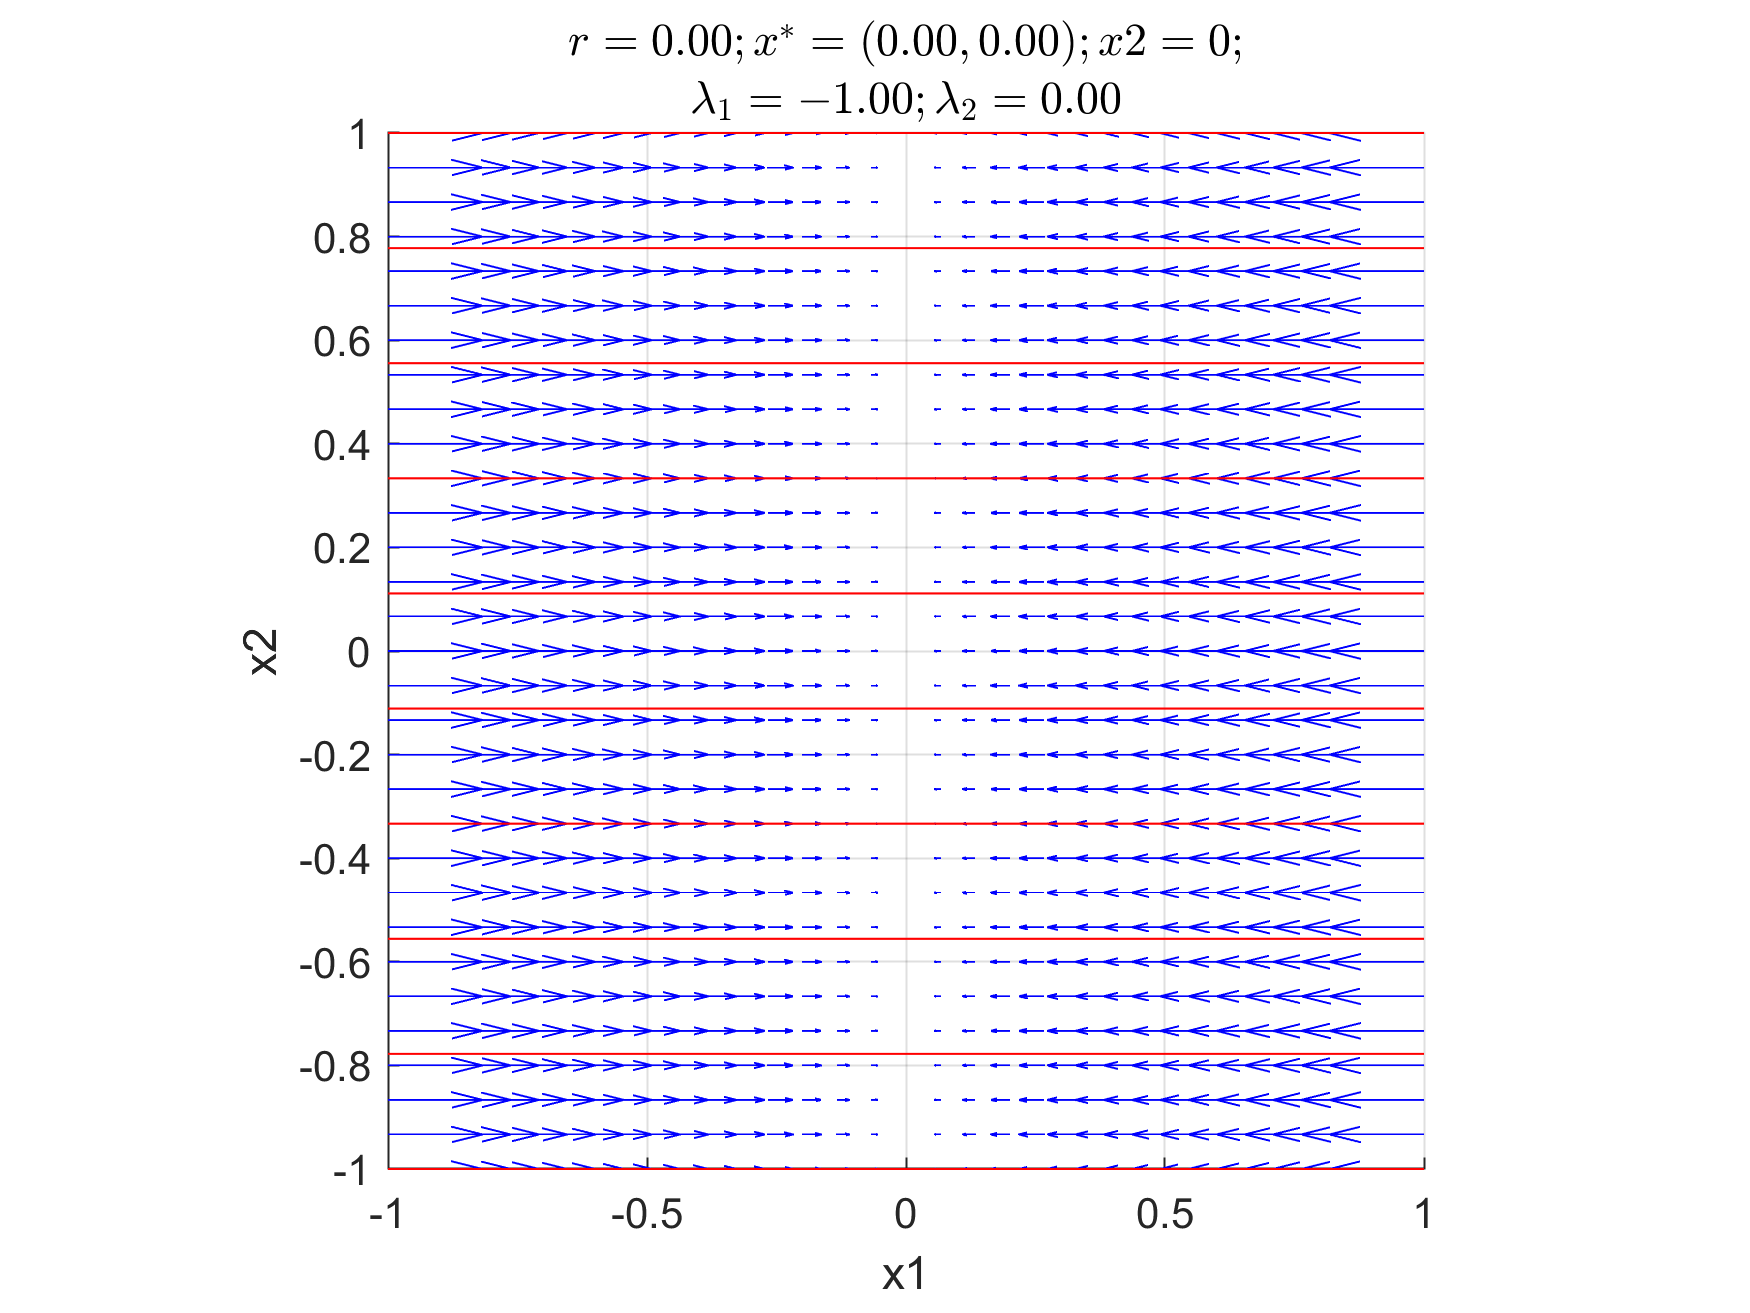
\includegraphics[width=\linewidth, trim={1cm, 0, 1cm, 0}, clip]{x1r0-lin.png}
            \caption{Линеаризованная система}
        \end{subfigure}
        \caption{Фазовые диаграммы}
    \end{figure}

    Для~(\ref{J23}) положение равновесия имеет тип
    \paragraph*{Седло} $r < \dfrac{1}{4},\,(\lambda_{1, 2} \in \R; \lambda_1\cdot\lambda_2 > 0)$\nopagebreak
    \begin{figure}[H]
        \begin{subfigure}{0.5\linewidth}
            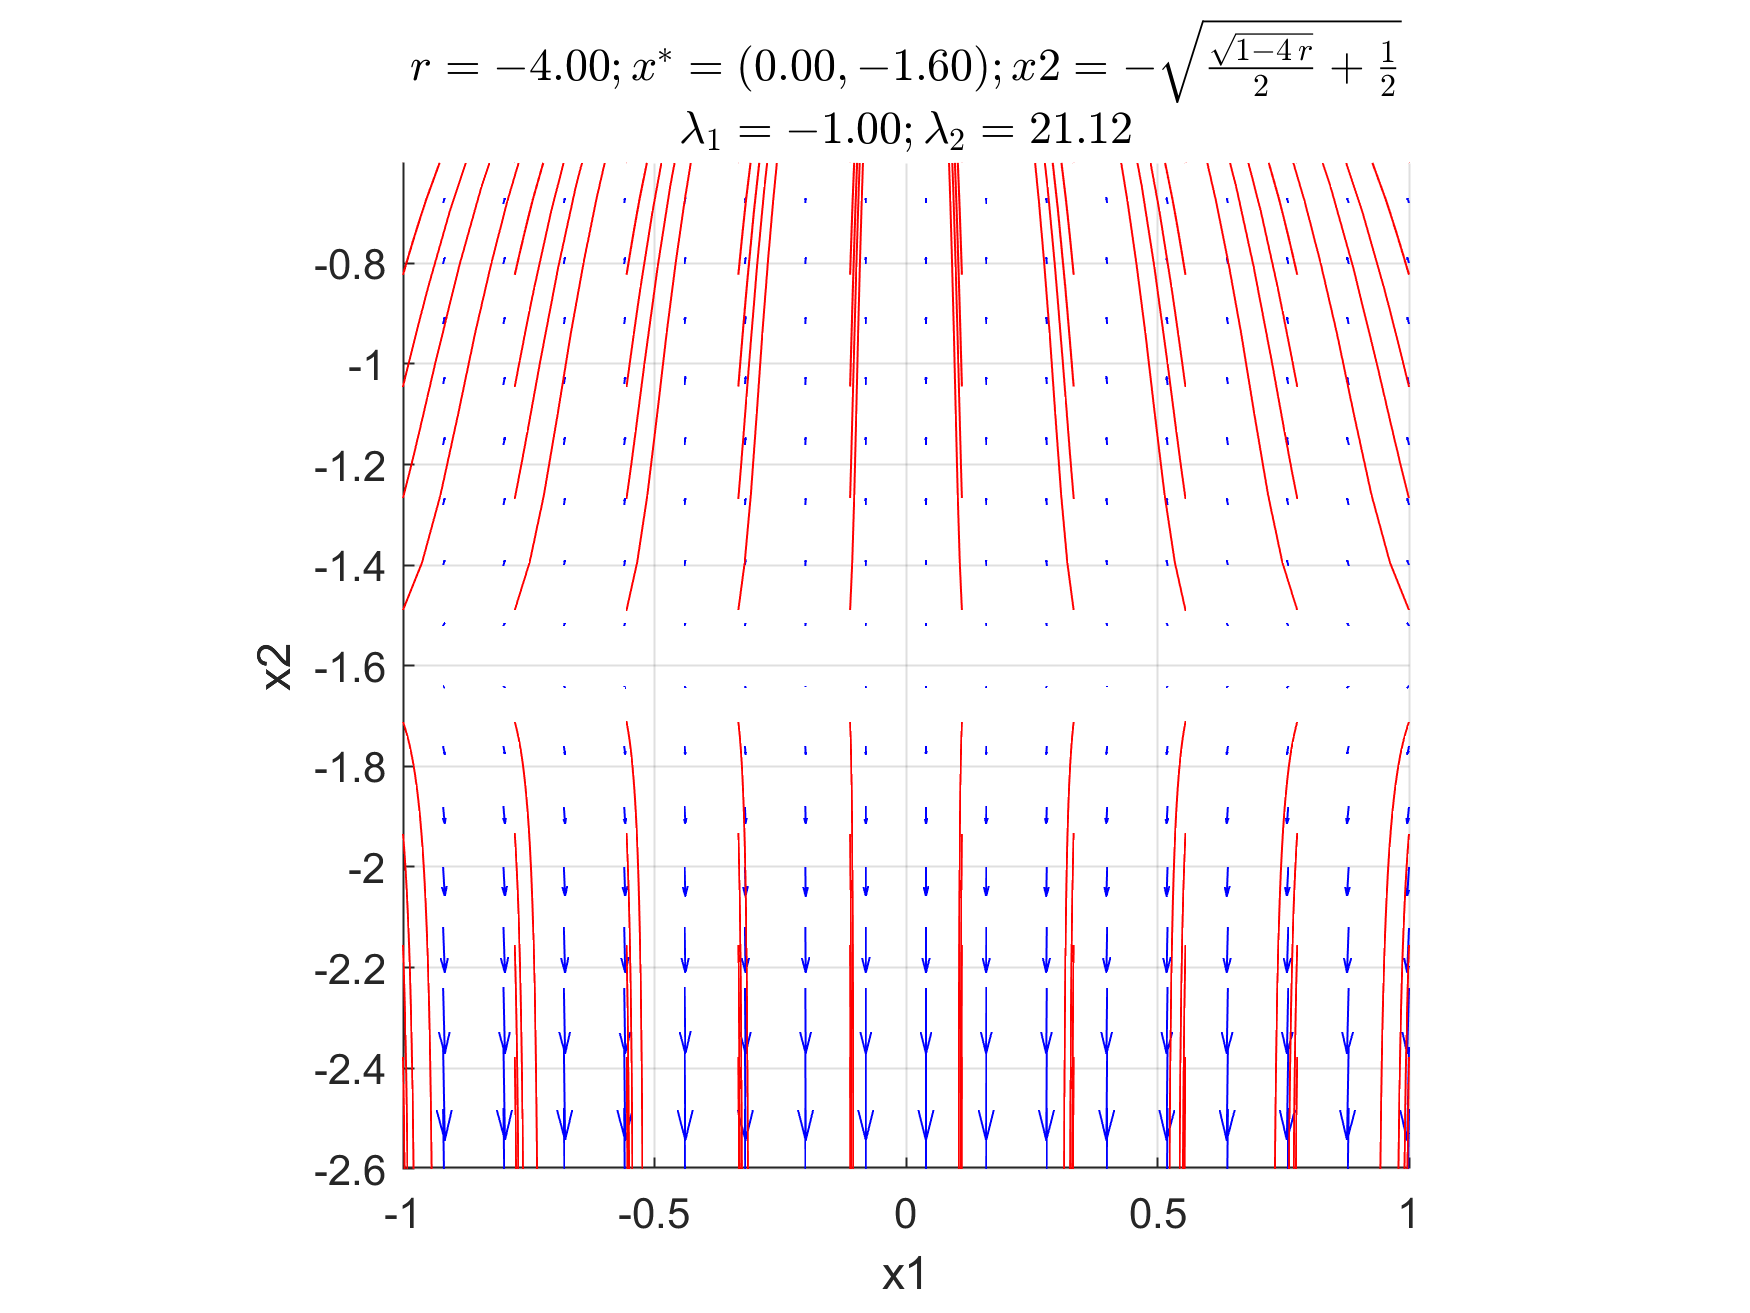
\includegraphics[width=\linewidth, trim={1cm, 0, 1cm, 0}, clip]{x23r-4.png}
            \caption{Исходная система}
        \end{subfigure}
        \begin{subfigure}{0.5\linewidth}
            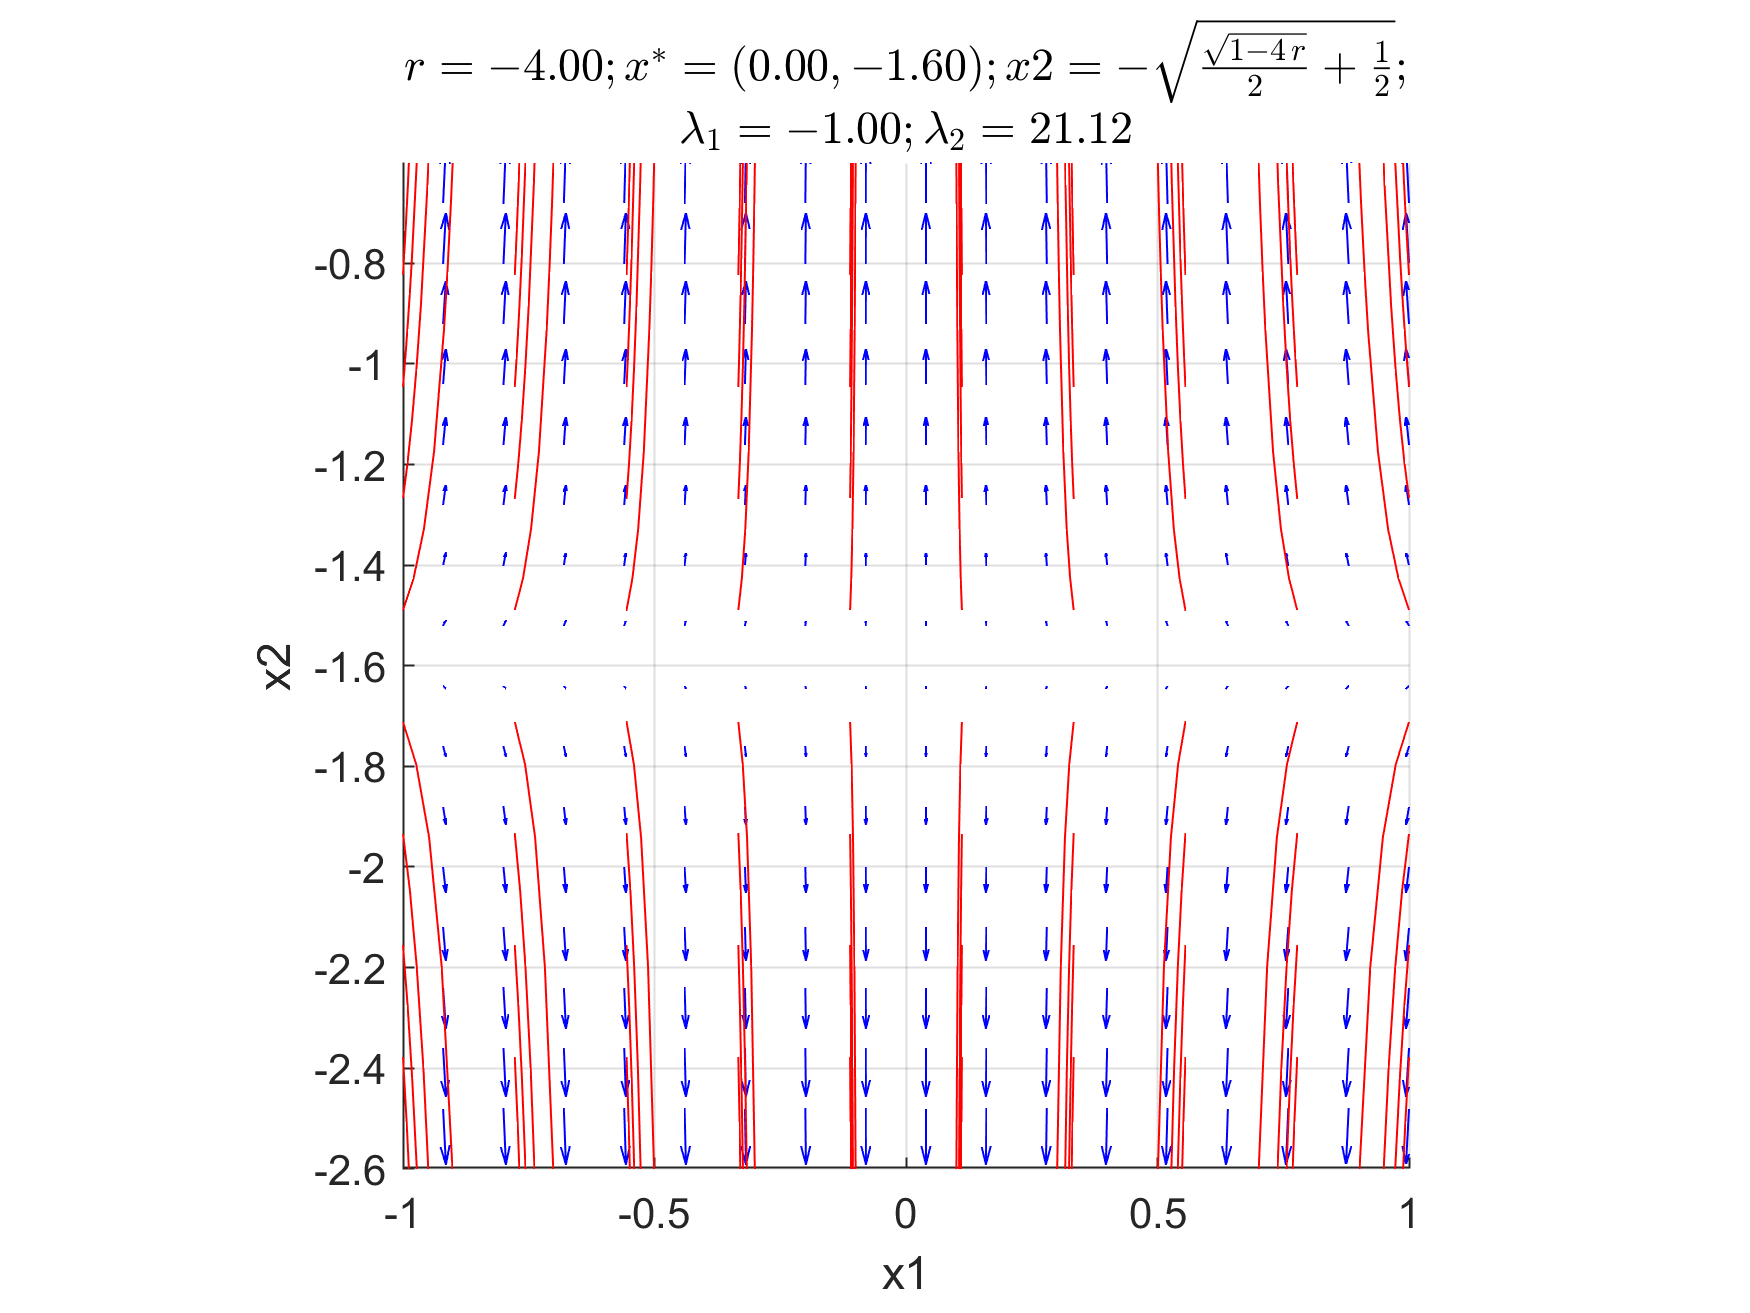
\includegraphics[width=\linewidth, trim={1cm, 0, 1cm, 0}, clip]{x23r-4-lin.png}
            \caption{Линеаризованная система}
        \end{subfigure}
        \caption{Фазовые диаграммы}
    \end{figure}

    \paragraph*{Вырожденный случай}  $r = \left\{\dfrac{1}{4} \right\},\,(\lambda_2 = 0 )$\nopagebreak
    \begin{figure}[H]
        \begin{subfigure}{0.5\linewidth}
            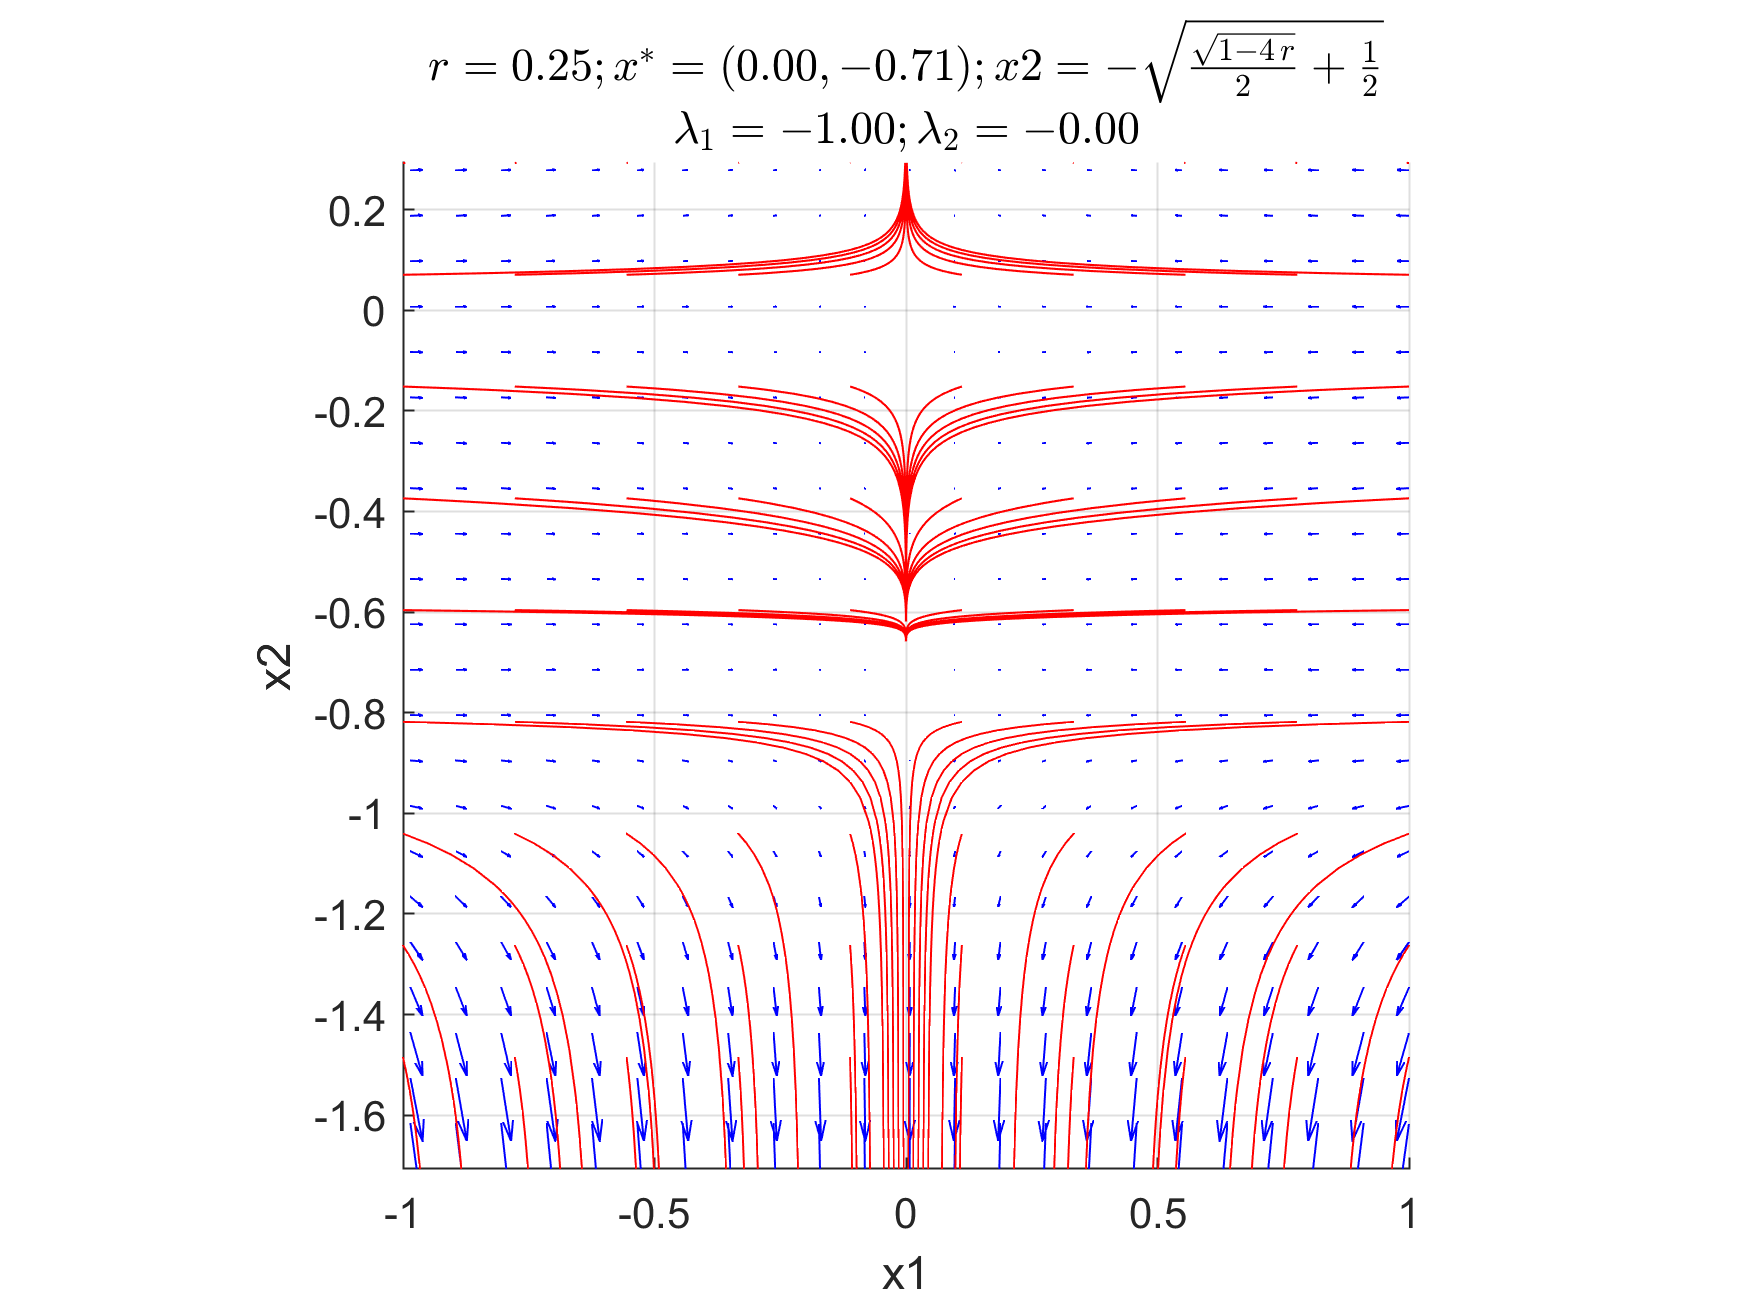
\includegraphics[width=\linewidth, trim={1cm, 0, 1cm, 0}, clip]{x23r025.png}
            \caption{Исходная система}
        \end{subfigure}
        \begin{subfigure}{0.5\linewidth}
            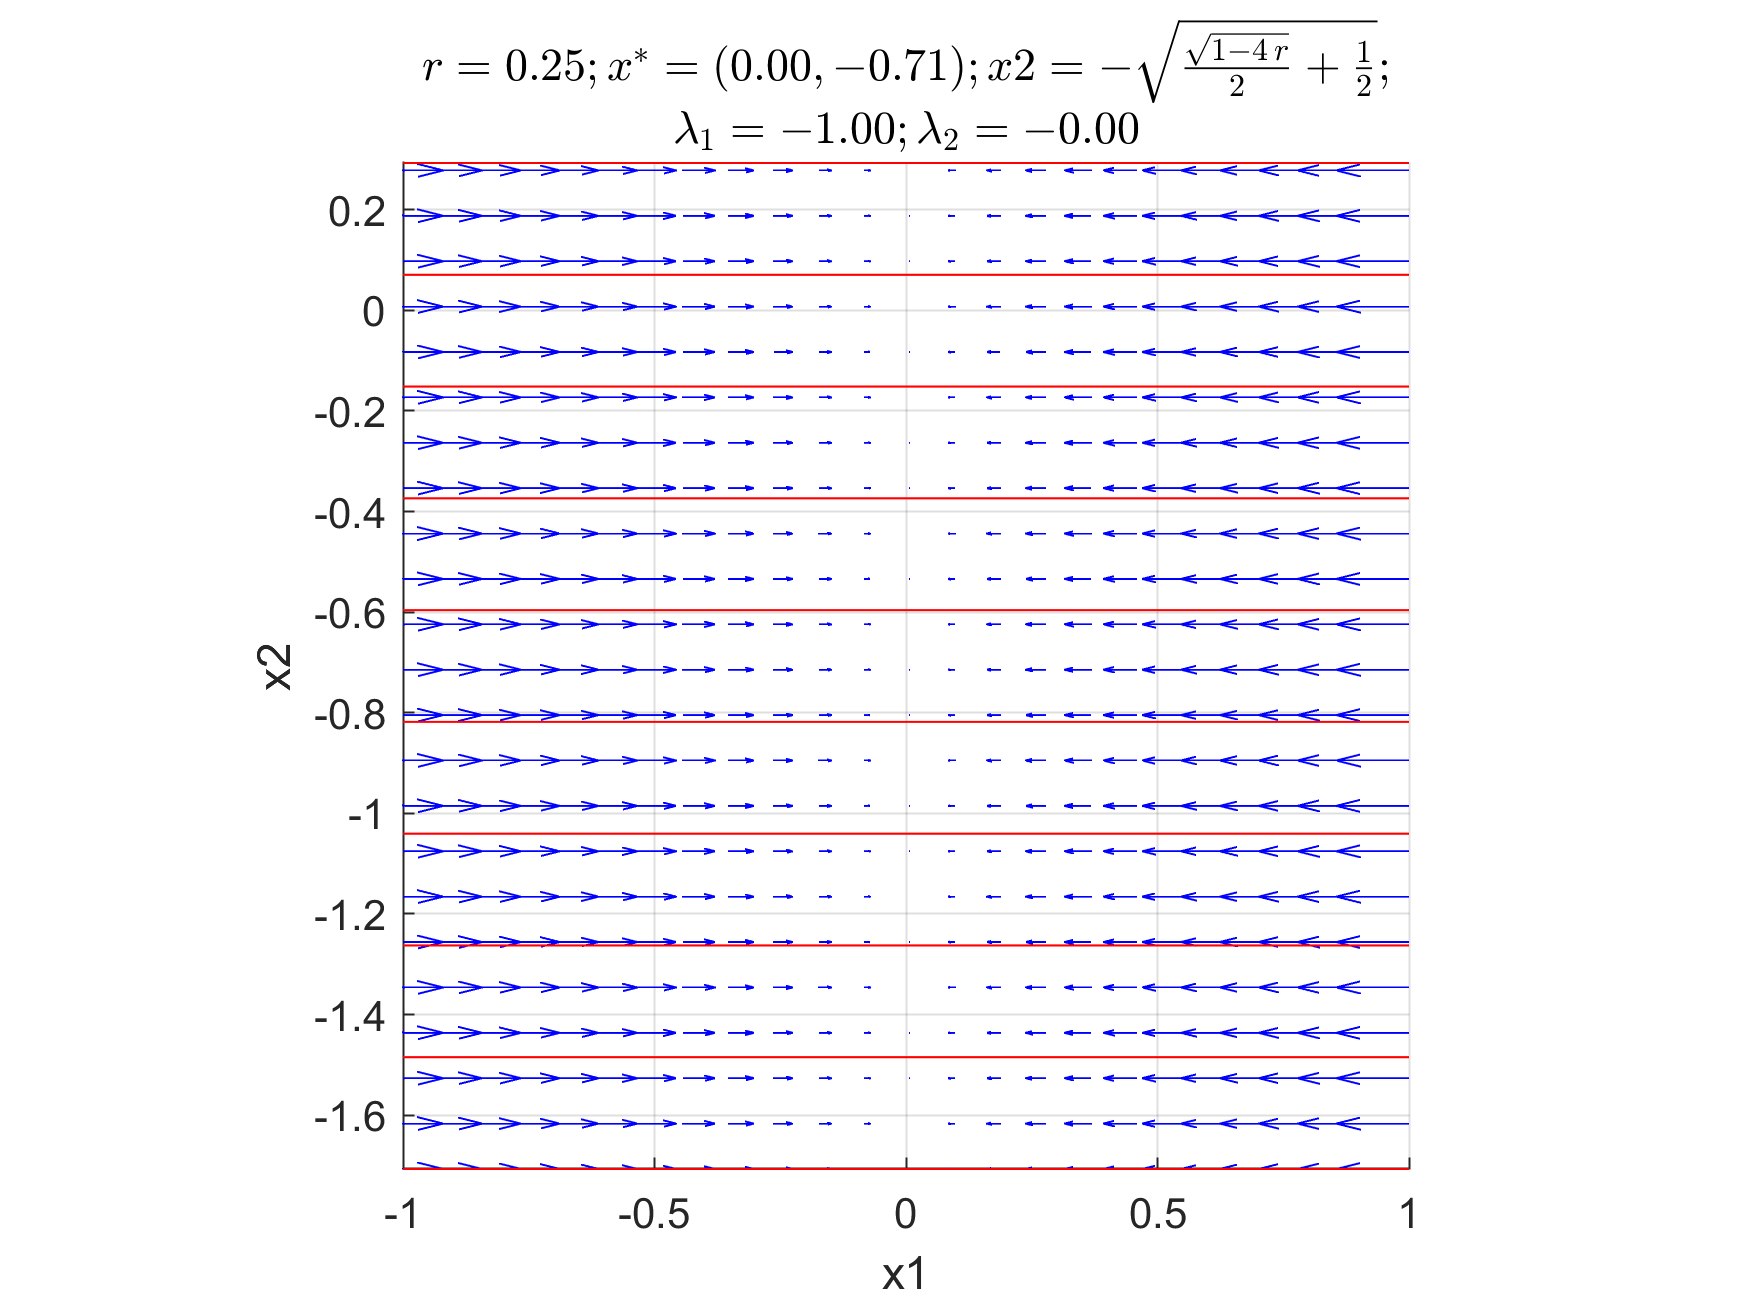
\includegraphics[width=\linewidth, trim={1cm, 0, 1cm, 0}, clip]{x23r025-lin.png}
            \caption{Линеаризованная система}
        \end{subfigure}
        \caption{Фазовые диаграммы}
    \end{figure}

    Для~(\ref{J45}) положение равновесия имеет тип
    \paragraph*{Устойчивый узел} $0 < r < \dfrac{1}{4},\,(\lambda_{1, 2} \in \R; \lambda_1\cdot\lambda_2 > 0)$\nopagebreak
    \begin{figure}[H]
        \begin{subfigure}{0.5\linewidth}
            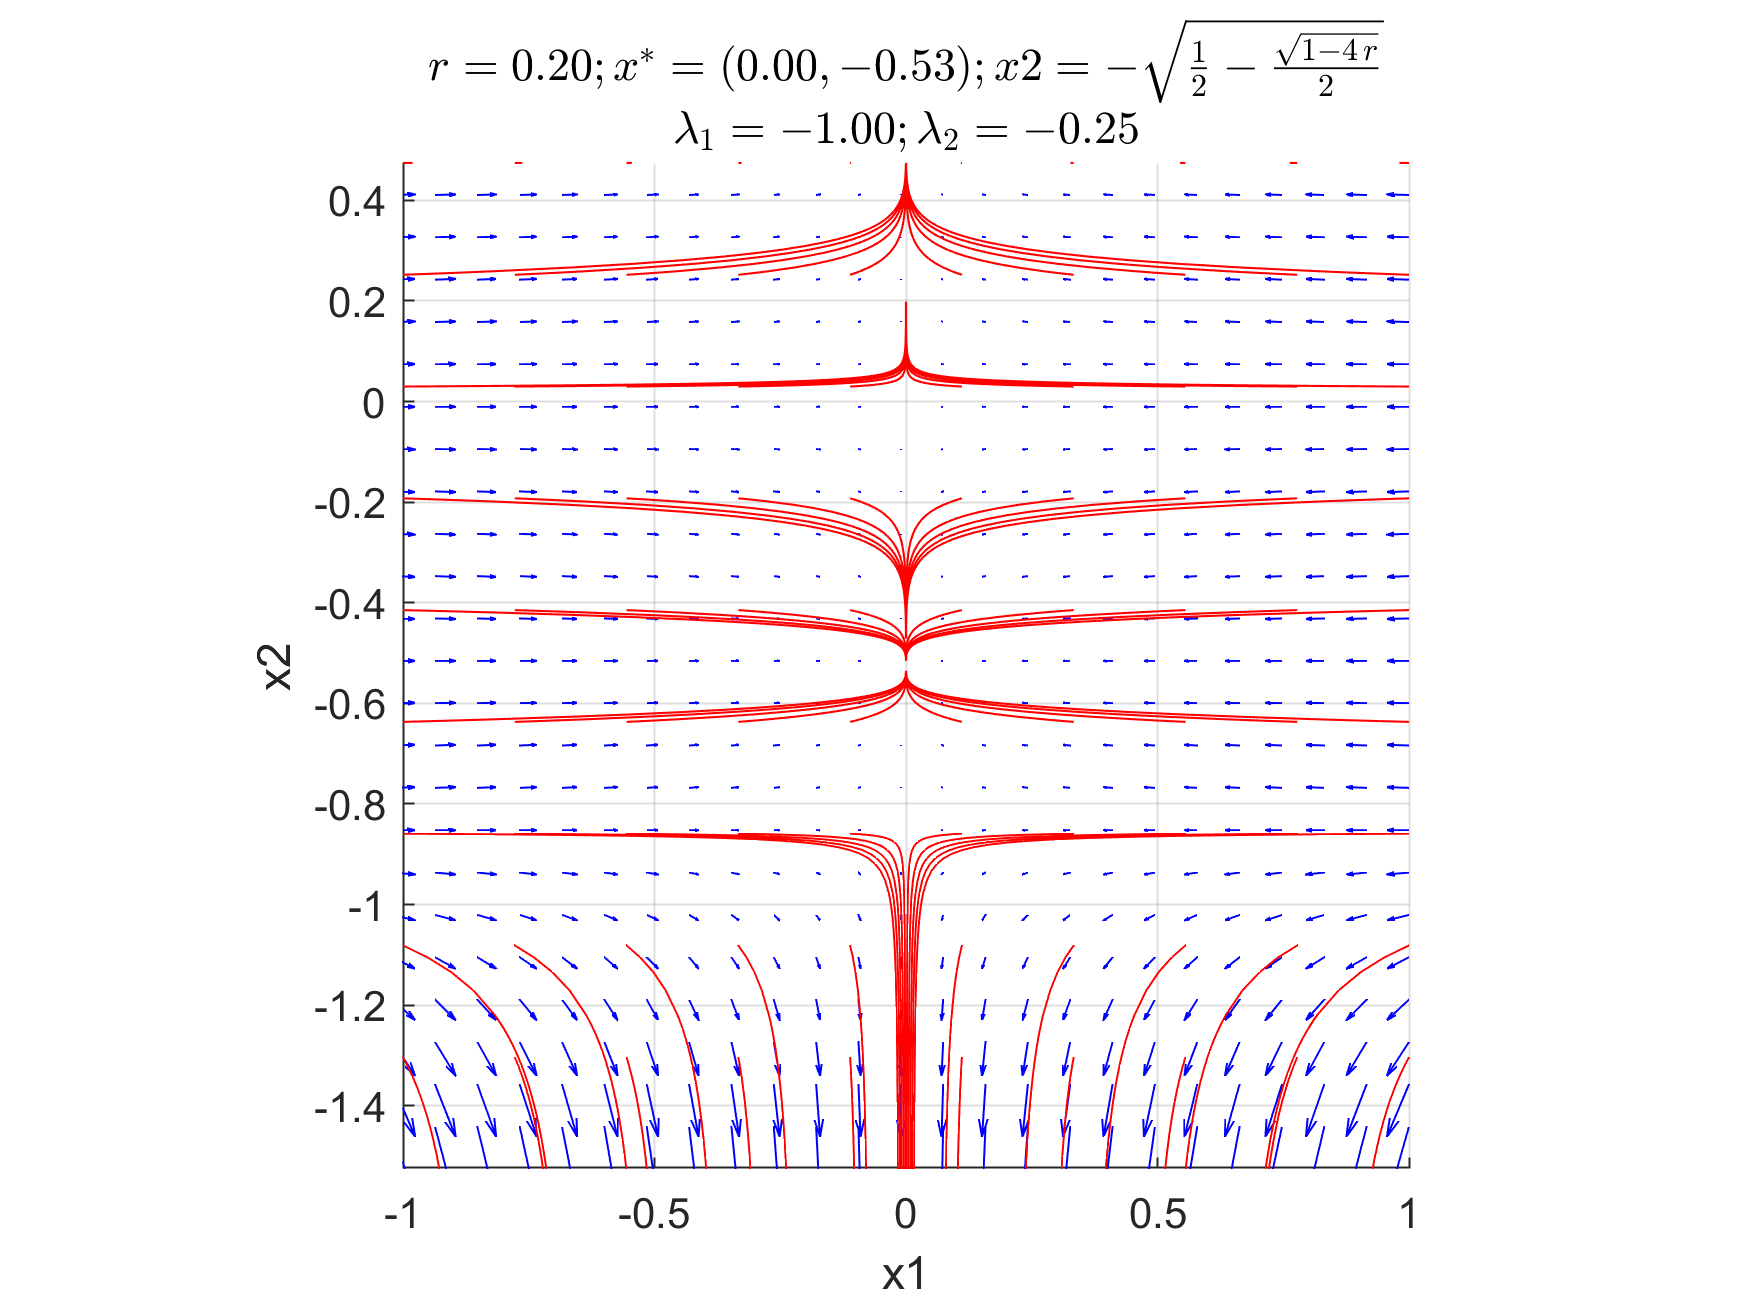
\includegraphics[width=\linewidth, trim={1cm, 0, 1cm, 0}, clip]{x45r02.png}
            \caption{Исходная система}
        \end{subfigure}
        \begin{subfigure}{0.5\linewidth}
            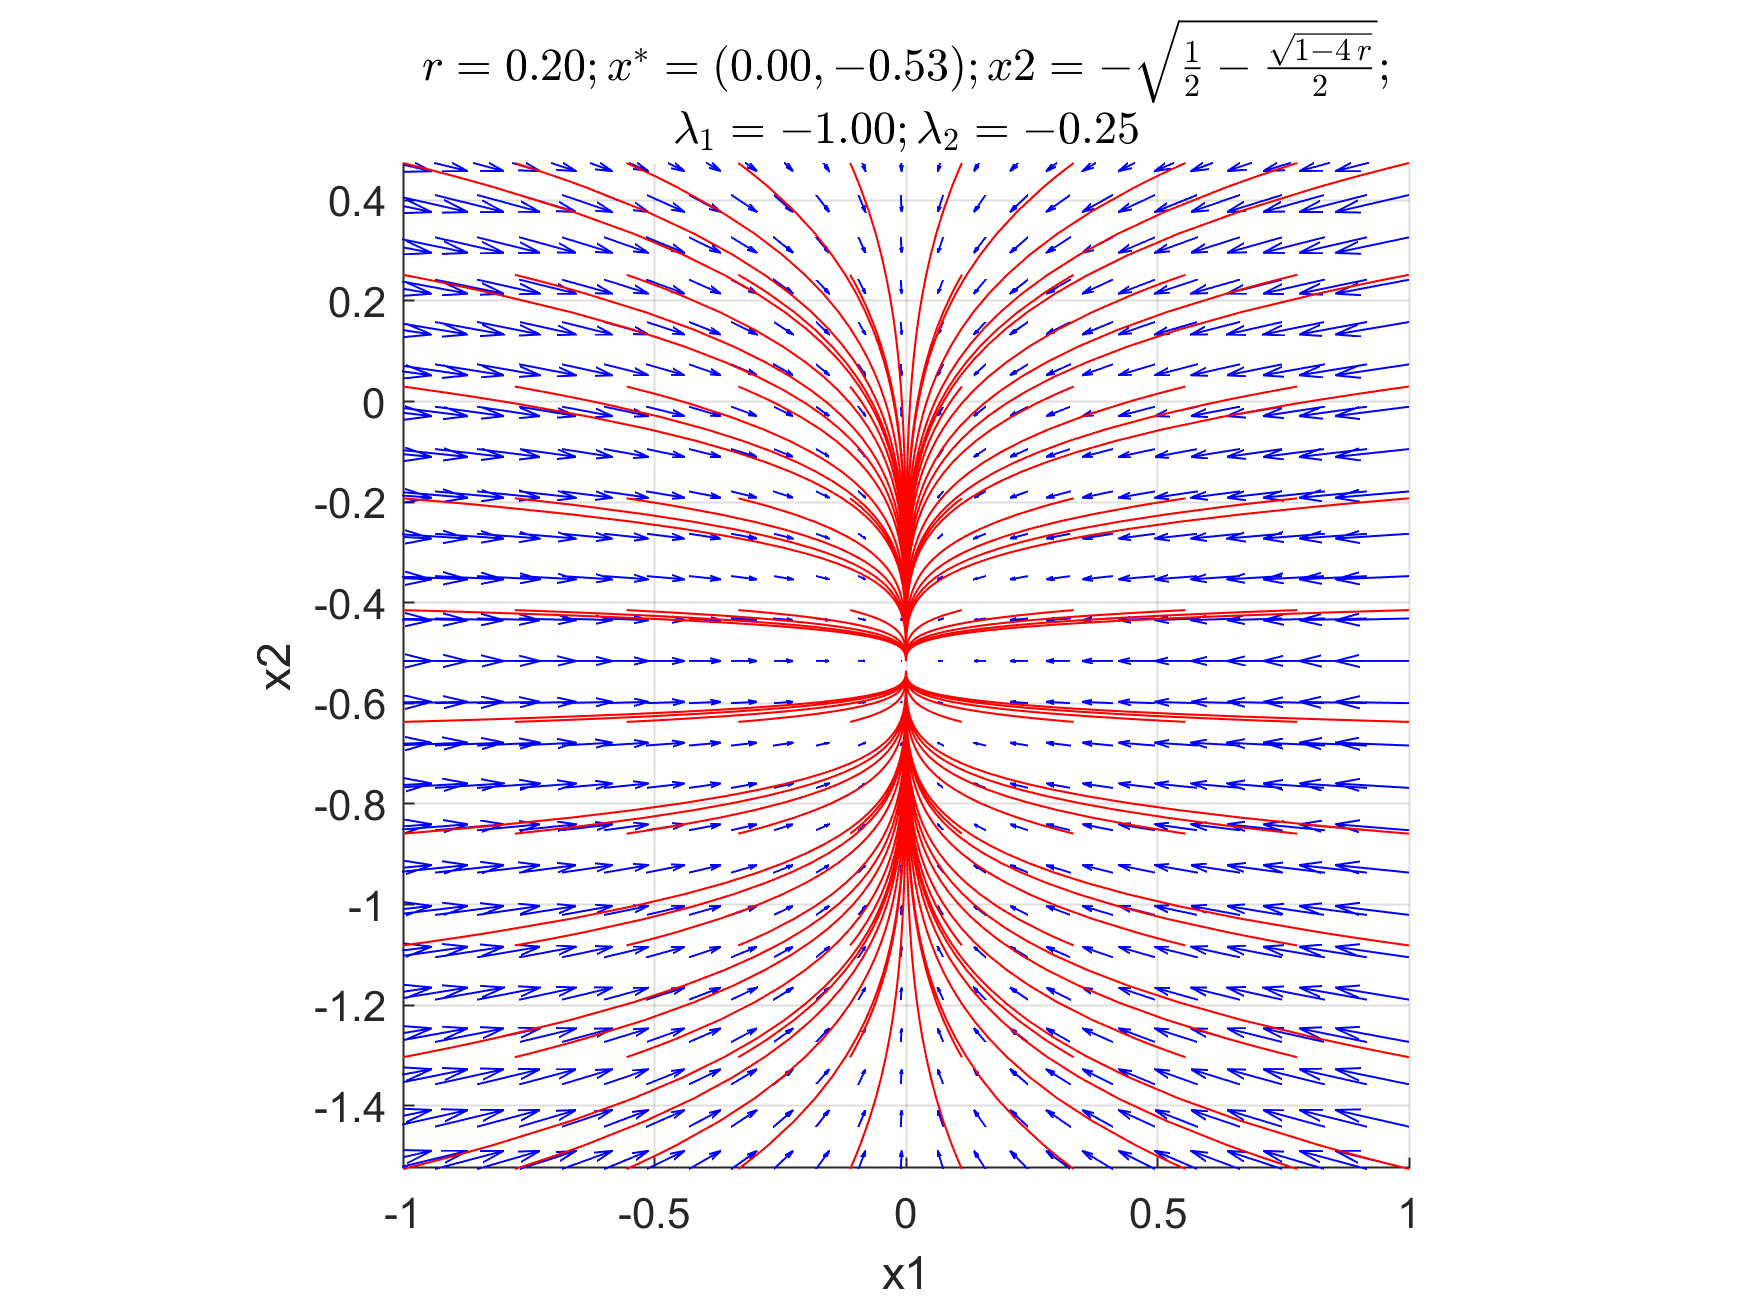
\includegraphics[width=\linewidth, trim={1cm, 0, 1cm, 0}, clip]{x45r02-lin.png}
            \caption{Линеаризованная система}
        \end{subfigure}
        \caption{Фазовые диаграммы}
    \end{figure}

    \paragraph*{Вырожденный случай} $r = \left\{0,\, \dfrac{1}{4} \right\},\,(\lambda_2 = 0$\nopagebreak
    \begin{figure}[H]
        \begin{subfigure}{0.5\linewidth}
            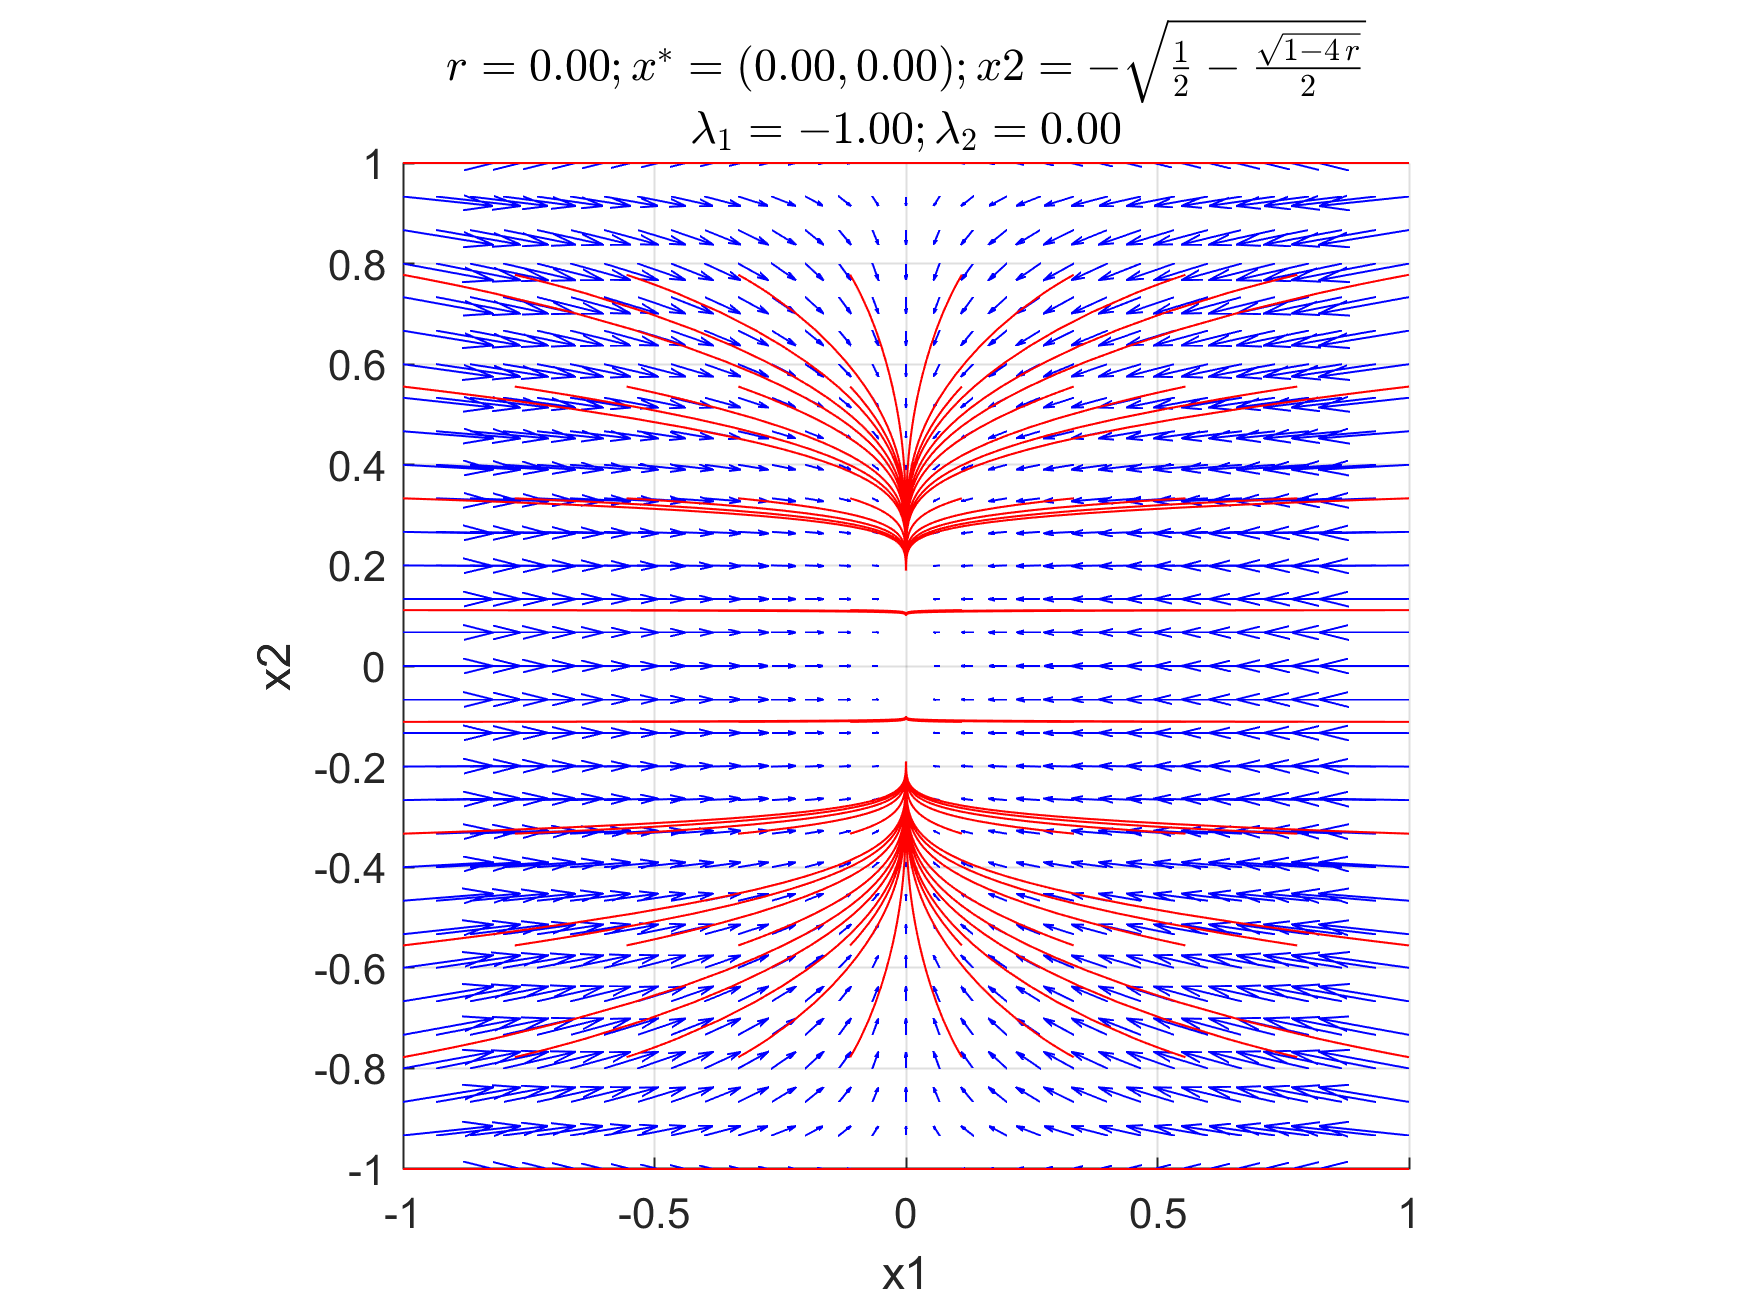
\includegraphics[width=\linewidth, trim={1cm, 0, 1cm, 0}, clip]{x45r0.png}
            \caption{Исходная система}
        \end{subfigure}
        \begin{subfigure}{0.5\linewidth}
            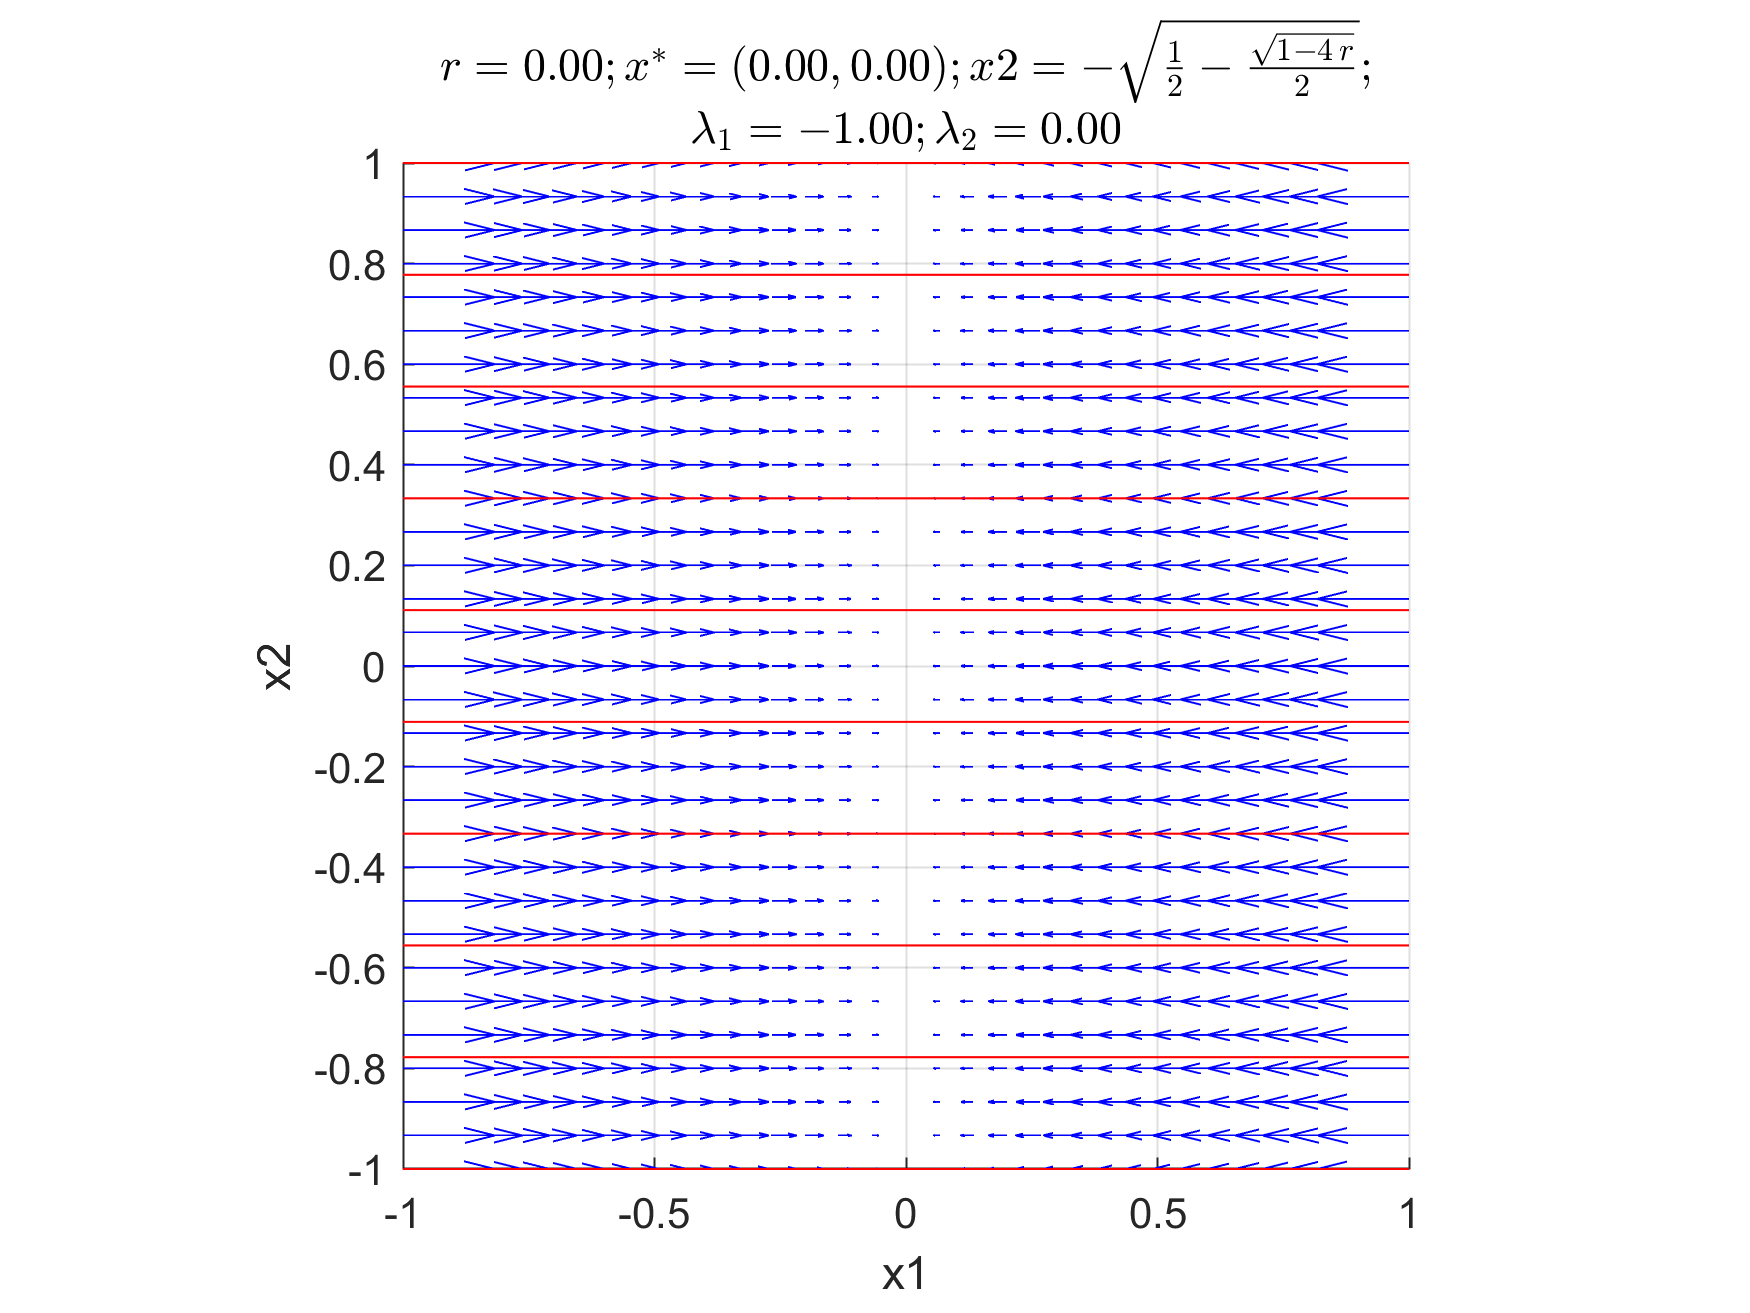
\includegraphics[width=\linewidth, trim={1cm, 0, 1cm, 0}, clip]{x45r0-lin.png}
            \caption{Линеаризованная система}
        \end{subfigure}
        \caption{Фазовые диаграммы}
    \end{figure}

    \section*{Вывод}
    В работе исследована динамика нелинейной системы и найдены следующие изменения динамики:
    \begin{itemize}
        \item Седлоузловая бифуркация для положения~\eqref{p1} при $r = 0$
        \item Для положений~\eqref{p2}--\eqref{p5} за пределами указанного диапазона значений $r$ нет положений равновесия
        \item На краях диапазона положений \eqref{p2} - \eqref{p5} система вырождается
    \end{itemize}


\end{document}
